%
% sample.tex
% $Id: sample.tex,v 1.1 2006/03/18 00:21:36 johnh Exp johnh $
%
% File is renamed to sensys-full.tex to reflect the twists made to use sensys-proc.cls.
%

% The default of sigplan-proc-varsize is 9pt, indented paragraphs (acm style)
% For Sensys or other 10pt conference, use the 10pt option
%\documentclass{sigplan-proc-varsize}
% options:
%\documentclass[9pt]{sigplan-proc-varsize}
%\documentclass[nocopyrightspace,10pt]{sigplan-proc-varsize-sensys-abstract}

%\documentclass[10pt]{sensys-proc}
\documentclass[10pt,abstract]{sensys-proc}

% % hack to avoid the ugly ACM paragraph definition
% % => can't leave blank line after this
% (remove comment for this hack)
% \renewcommand{\paragraph}[1]{\vskip 6pt\noindent\textbf{#1 }}

\usepackage{graphicx}
\usepackage{subfigure}
\usepackage{cite}
\usepackage{url}
\usepackage{slashbox}
\usepackage{curves}
\usepackage{algorithmic}
\usepackage{algorithm}
\usepackage{balance}
\usepackage{soul}
\graphicspath{{pictures/}}
\usepackage{balance}
\usepackage{comment}
\usepackage{amsmath}
\usepackage{amssymb}
\usepackage{amsfonts}

\usepackage[pass,letterpaper]{geometry}

\author{
%
% The command \alignauthor (no curly braces needed) should
% precede each author name, affiliation/snail-mail address and
% e-mail address. Additionally, tag each line of
% affiliation/address with \affaddr, and tag the
%% e-mail address with \email.
Mingmin Zhao, Ruipeng Gao, Jiaxu Zhu, Tao Ye, Fan Ye, Yizhou Wang, Kaigui Bian, Ming Zhang \\
\affaddr{Department of Electrical Engineering and Computer Science}\\
\affaddr{Peking University, Beijing, China}\\
\email{\{zhaomingmin, gaoruipeng, zhujiaxu, yetao, yefan, Yizhou.Wang, bkg, mzhang\}@pku.edu.cn}
}

\title{Poster Abstract: VeLoc: Finding Your Car in the Parking Lot}

\crdata{978-1-4503-1169-4}
\conferenceinfo{SenSys'14,} {November 3--6, 2014, Memphis, TN, USA.}
\CopyrightYear{2014}

\renewcommand{\baselinestretch}{1.08}
\begin{document}

\maketitle

\begin{abstract}\label{sec:abstract}
Remembering where a vehicle was parked has proven a hassle in large parking structures. Existing RF signature based indoor localization technology is not applicable where such signals may not be available such as at underground parking lots.
Instrumenting additional sensors may solve the problem but at the cost of significant overheads in time, money and human efforts. In this paper, we propose VeLoc, a smartphone-based vehicle localization approach that tracks the vehicle's parking location using the embedded accelerometer and gyroscope sensors.
It harnesses constraints imposed by the map and landmarks (e.g., speed bumps) recognized from inertial data, employs a Bayesian filtering framework to estimate the location of the vehicle. It is also robust to different orientations of the phone relative to the vehicle, and even jolting during bumpy rides. We have conducted extensive experiments in 3 parking lots of different sizes and structures, using 3 vehicles and 3 kinds of driving styles. We find that VeLoc can always localize the vehicle within $10m$, which is sufficient for the driver to trigger a honk using the car key. This is achieved even when the initial position and heading direction of the vehicle is unknown.


%(xx what other performance numbers or nice features can we boast?)


% a in lacking unique features While WiFi-based indoor localization is attractive, there are many indoor places without WiFi coverage but also show strong demand for localization. This paper describes a system and associated algorithms to address the indoor vehicle localization problem without installation of additional infrastructure. In this system, which we call the \textbf{VeLocE}, we utilize the sensor data of smartphones in the vehicle together with the floor map of the parking lot to track the vehicle. VeLocE simultaneously harness constraints imposed by the map and environment sensing. All these cues are codified into a novel Augmented Particle Filtering framework to estimate the position of the vehicle. Experimental results show that VeLocE performs well even the initial position and the initial heading direction of the vehicle is absolutely unknown.
\end{abstract}



\category{H.5.2}{Information Interfaces and Presentation}{User Interfaces}
\category{H.1.2}{Models and Principles}{User/Machine Systems}[Human Information Processing]
\category{I.5.1}{Pattern\break Recognition}{Models}[Neural Nets]

\keywords{Vehicle Localization, Indoor Localization, Inertial Tracking, Robotic Navigation, Virtual Landmarks}

\section{Introduction}
Remembering where a vehicle was parked has proven a hassle in large parking structures. Existing RF signature based indoor localization technology is not applicable where such signals may not be available such as at underground parking lots.
Instrumenting additional sensors may solve the problem but at the cost of significant overheads in time, money and human efforts. 

\iffalse
(Problem)
With the rapid growth of personal vehicles amount and growth of urban parking spaces demands, there appear numerous large parking facilities, most of which are built underground. Drivers may find it a nightmare to search for their vehicles in the dim and mazelike parking lot since the parking lots are very large and have similar appearance inside without visual features.

(Why it's hard to solve) Localizing a vehicle in a parking lot is a challenging problem due to the special environment most parking lots have. Although most vehicles are equipped with vehicle-mounted GPS and the mobile devices of the driver also have GPS, the indoor environment especially underground environment makes it impractical to use GPS. Radio Frequency (RF) fingerprinting of WiFi signals which has been a popular approach to indoor localization \cite{bahl00radar, youssef2005horus} do not work here since the poor WiFi coverage in the parking lots. An optional solution is to install additional infrastructure(e.g. sensor network), however, this method is effort-intensive and costly, also, this kind of installation may be infeasible in many parking lots already built.
\fi

%An ideal solution should work without the aid of such additional environmental sensors, and it should provide accurate enough location of the vehicle to the driver even where GPS and RF signals are weak or unavailable. Only then can it be applicable to general enough scenarios such as underground and legacy parking lots.


%(Ideal solution)
%Common used smartphone is an ideal choice to address this problem. Inertial sensors inside the smartphone can provide cues for localization vehicles. If the result of localization can be recorded on the smartphone, the driver could use his smartphone to find his car when he comes back. In addition, informing drivers the map of the parking lot and the real-time position of the vehicle would be helpful for drivers to search for an unoccupied parking place especially in an unfamiliar environment.

%(Effects)

%In this paper, we propose 
VeLoc is a vehicle localization system that utilizes accelerometer and gyroscope sensors in the smartphone to provide accurate vehicle localization. It does not rely on GPS or RF signals, neither require any additional sensors to instrument the parking ground. %Instead, the driver simply runs the VeLoc application before entering a parking structure. VeLoc will track the vehicle movements, estimate its location, and record where the vehicle is finally parked.% This information is then used to direct the driver back to the parked spot when she/he returns.

%The intuition behind VeLoc is that although a noisy trajectory does not, by itself, reveal a vehicle's location, using the constraints imposed by the parking structure��s map and detected landmarks is able to help vehicle tracking(shown in Figure \ref{fig_poster}).
%This is because (a) trajectories can be used for localization since only a few paths on the map could accommodate the trajectory. (b) once a landmark is detected, only a few positions marked with the same kind of landmark are possible. (c) using both map constraints and detected landmark could narrow down the uncertainty more quickly and trace a vehicle more accurately.
%This is because (i) there may be only a few paths on the map that could accommodate the trajectory as shown in Figure \ref{fig_apf_intuition1}.
%(ii) A detected landmark (e.g., a bump, turning or slope) can further pin down the positions where a vehicle might be (as shown in Figure \ref{fig_apf_intuition2}) since there are limited number of such landmarks on the map. Hence, using the synergy of both constraints is able to narrow down the uncertainty more quickly and trace a vehicle more accurately (as shown in Figure \ref{fig_apf_intuition3}).


%We design several algorithms and implement a real-time system to localize a vehicle using a smartphone inside with arbitrary pose and possible jolting. No installation of additional infrastructure is needed and all what users need to do during a drive is to run the VeLoc to process collected data. Finally, VeLoc provides localization result for usrs to find their car when they come back latter.

%(Difficulties)
Realizing such an inertial-based solution, however, involves non-trivial challenges. First, the driver may place the phone in arbitrary positions and road conditions may jolt the phone to change its position on the course. How to estimate the pose (i.e., the relative orientation of the smartphone to the vehicle) despite all such uncertainty and disturbances? Second, %although admirable work has been done~\cite{ParkSense,Lindqvist:Undistracted_Driving} to estimate the walking distance of a person,
inferring the vehicle's traveling distance or even trajectory is still difficult due to the lack of periodic acceleration patterns, which are fundamental in step-counting techniques~\cite{ParkSense,Lindqvist:Undistracted_Driving}. %Although landmarks of unique acceleration, magnetism patterns such as escalators can calibrate the location~\cite{Wang:UnLoc},
Also, identifying which types of landmarks can be reliably recognized despite different parking lots, vehicles and driving styles, and how, remain open questions. Finally, since both the pose and landmark detection results contain errors, how can one track the location of a vehicle accurately, such that the driver can always find the vehicle? % tracking the vehicle in real time requires efficient computation that can fit the resources available on smartphones.

%(High-level description)
%VeLoc contains several components to deal with the above challenges.
%A \textit{Pose estimation} algorithm estimates the pose of the smartphone inside the vehicle, regardless of how the phone is oriented relative to the vehicle and occasional changes in its pose due to bumpy driving. We also develop a \textit{Landmark detection} algorithm which uses pattern recognition and machine learning techniques~\cite{} to find unique patterns corresponding to different types of landmarks and implement real-time classification algorithm to detect them reliably.
%Finally, we represent the uncertainty about the state of the vehicle explicitly as probability distributions. We incorporate the uncertainty arising from sensing and the parking structure's map information provided by the map or detected landmarks, into a novel Bayes Filtering framework, specifically, \textit{ Augmented Particle Filtering} framework to simultaneously harness constraints imposed by the map and landmark detection for localization. (xx last sentence still too long and vague. need to sharpen the point)

%(High-level description)
As shown in Figure~\ref{pix:overview}, VeLoc contains three components to deal with the above challenges.
A \textit{pose estimation} module estimates the pose of the smartphone inside the vehicle. A \textit{landmark detection} module finds unique patterns corresponding to different types of landmarks and classify them reliably. A \textit{location estimation} module determines the vehicle's final location from the map and detected landmarks. 

\begin{figure}[h]
  \centering
  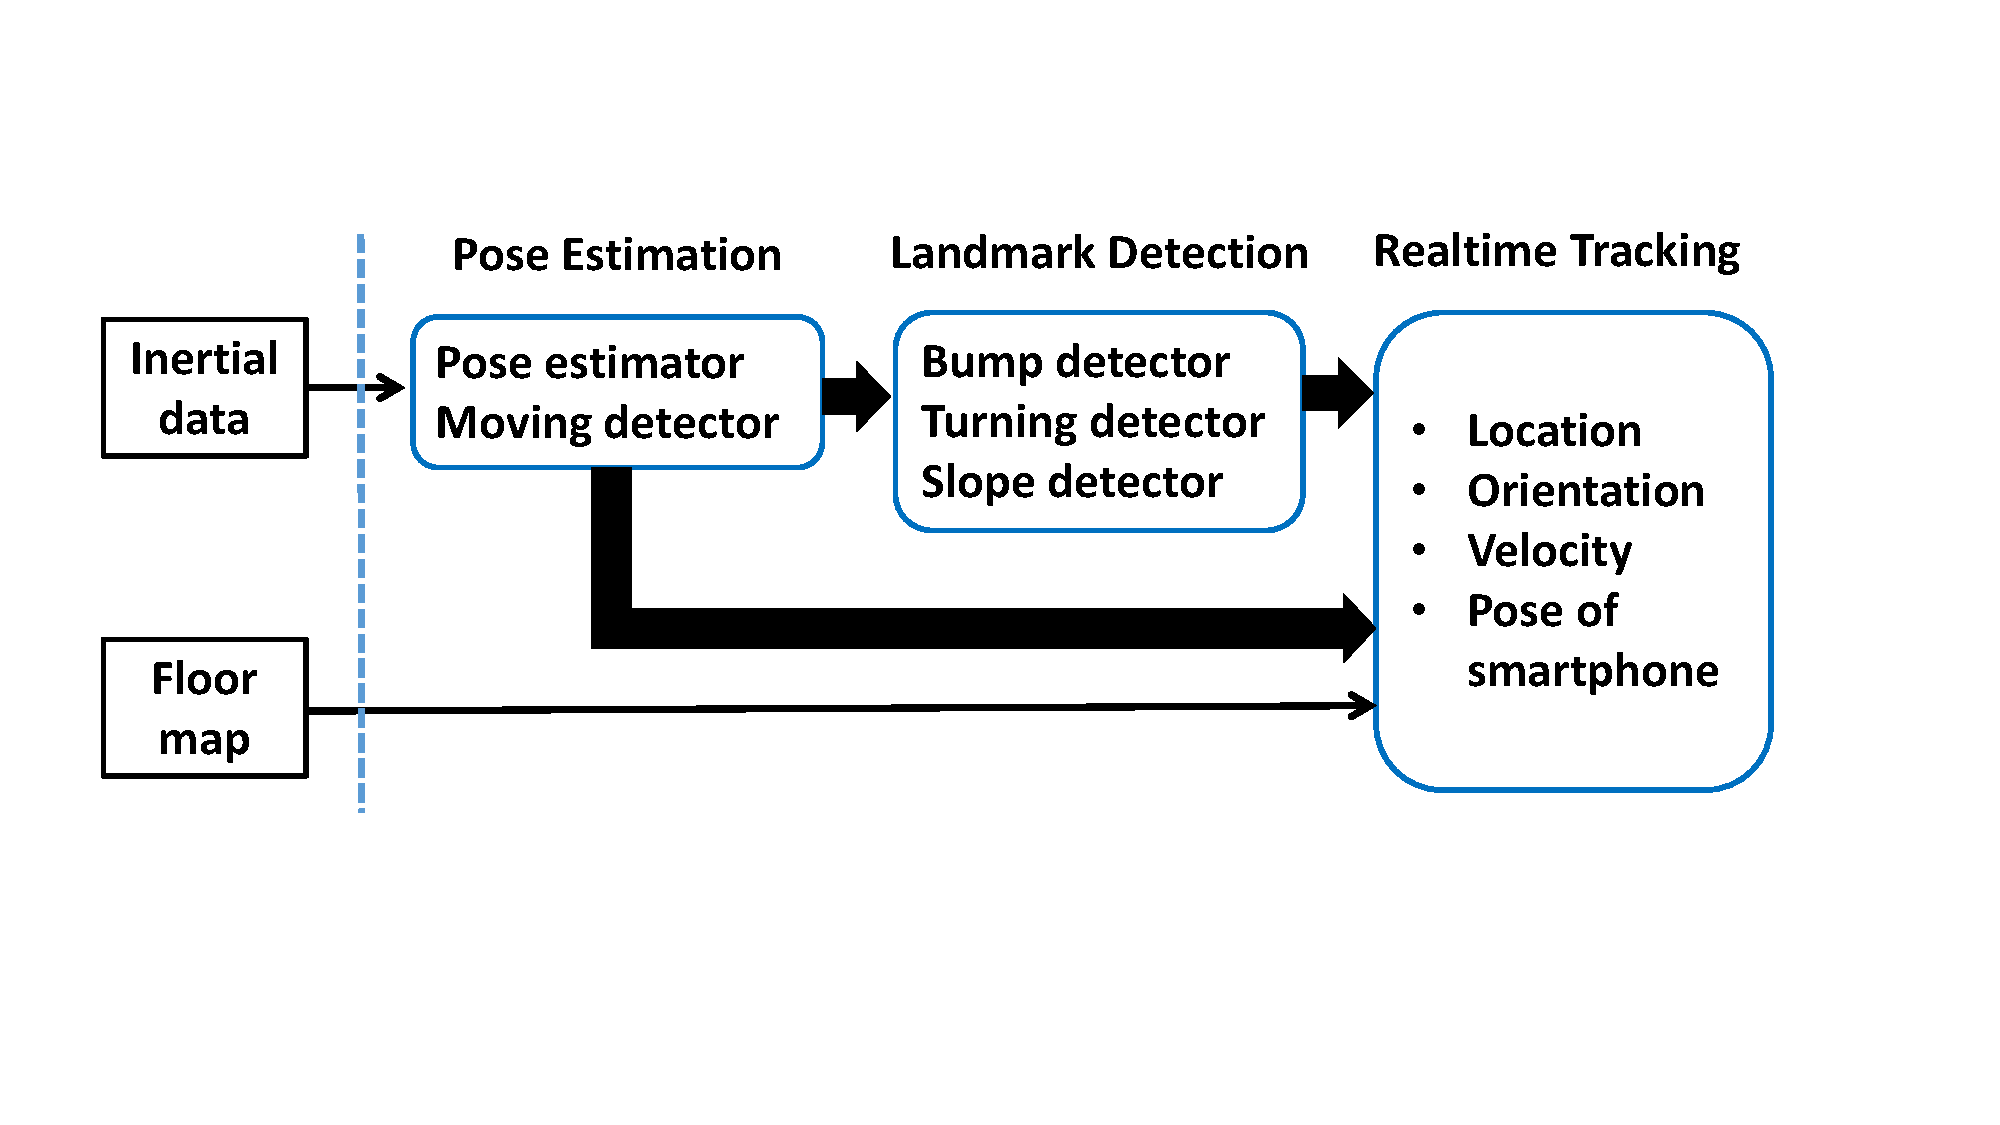
\includegraphics[width=0.5\textwidth]{overview}\\
  \caption{Three components of VeLoc. Inertial data is used to compute the smartphone's pose in the vehicle, then it is further processed to detect certain landmarks during driving, and the augmented particle filter harnesses constraints from landmark detection and the floor map for vehicle localization.}\label{pix:overview}
\end{figure}

\iffalse
Specifically, we make the following contributions in this work:

\iffalse
VeLoc contains several components to deal with the above challenges.
A \textit{pose estimation} module estimates the pose of the smartphone inside the vehicle, regardless of how the phone is oriented relative to the vehicle and occasional changes in its pose due to bumpy driving. We also develop a \textit{landmark detection} module which uses pattern recognition and machine learning techniques~\cite{} to find unique patterns corresponding to different types of landmarks and implement real-time classification algorithm to detect them reliably.
Finally, we design a novel Bayes Filtering framework, specifically, \textit{Augmented Particle Filtering} framework using probability distributions to represent the uncertainty about the state of the vehicle, which can be diminished by constraints imposed by the map and detected landmarks.
\fi

%Finally, we represent the uncertainty about the state of the vehicle explicitly as probability distributions. We incorporate the uncertainty arising from sensing and the parking structure's map information provided by the map or detected landmarks, into a novel Bayes Filtering framework, specifically, \textit{ Augmented Particle Filtering} framework to simultaneously harness constraints imposed by the map and landmark detection for localization. (xx last sentence still too long and vague. need to sharpen the point)


%(Contribution)

\begin{itemize}
  \item We develop a robust pose estimation algorithm that can handle arbitrary orientations of the phone in the vehicle and possible jolting that alters the pose during the course of driving. We identify a set of landmarks commonly encountered in parking structures, and propose respective detection algorithms to classify them reliably.
  \item We identify an opportunity to simultaneously harness constraints imposed by the parking structure's map and detected landmarks for localization. We formulate such constraints into a Bayes Filtering framework that uses probability distributions to represent the vehicle state, and infers the final location by reducing the uncertainty using the map and detected landmarks.
  \item We implement a prototype and conduct extensive experiments using different parking structures, vehicles and driving styles to evaluate the robustness and accuracy of VeLoc. We find that it can locate the vehicle within $10m$, which is sufficient for the remote key to trigger a honking sound. The pose can be estimated with 9 degrees error, which is fast enough to deal with occasional jolting in real time. % We also implement the algorithms in a smartphone app that can run in real time to track the vehicle's location, which demonstrate the computation efficiency of our design.
\end{itemize}

The rest of this paper is organized as follows: we give a brief design overview in Section~\ref{sec:overview}. We then propose a pose estimation algorithm for the smartphone inside a vehicle in Section~\ref{sec:pose}, and landmark detection algorithms in Section~\ref{sec:landmark}. Additionally, Section~\ref{sec:tracking} presents our sequential importance re-sampling framework. We report experimental evaluation in Section~\ref{sec:evaluation}, and review the related work in Section~\ref{sec:background}. After a discussion of limitations in Section~\ref{sec:discussion}, we conclude the paper in Section~\ref{sec:conclusion}.
\fi


The intuition behind VeLoc is that although a noisy trajectory does not, by itself, reveal a vehicle's location, using the constraints imposed by the parking structure��s map and detected landmarks is able to help vehicle tracking(shown in Figure \ref{fig_poster}).
%This is because (a) trajectories can be used for localization since only a few paths on the map could accommodate the trajectory. (b) once a landmark is detected, only a few positions marked with the same kind of landmark are possible. (c) using both map constraints and detected landmark could narrow down the uncertainty more quickly and trace a vehicle more accurately. 

\begin{figure}[h]
      \centering
      \vspace{-10pt}
        \subfigure[Localization using constraints imposed by the map.] {
        \begin{minipage}[b]{0.5\textwidth}
        \centering
        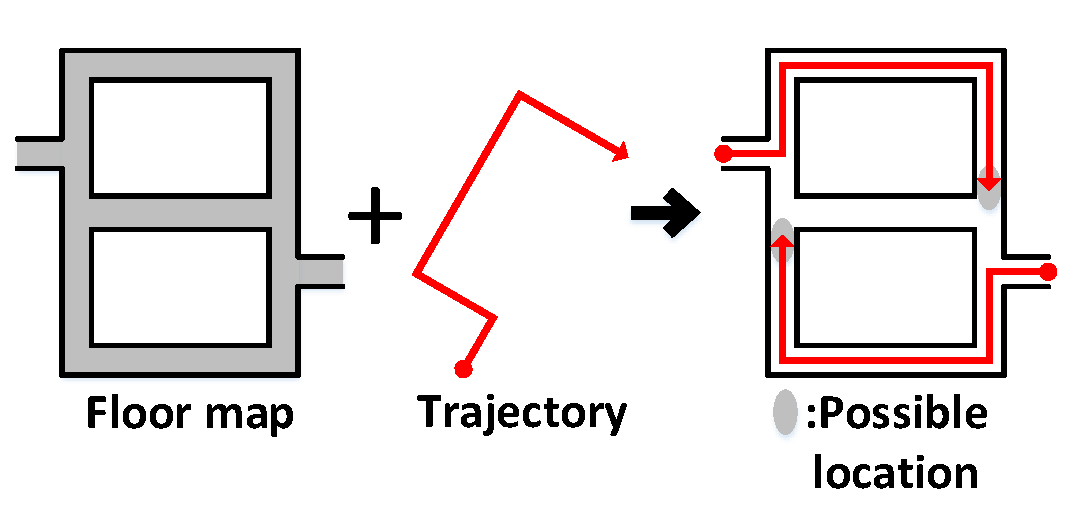
\includegraphics[width=0.8\textwidth]{apf1}\label{fig_apf_intuition1}
        \end{minipage}
        }
        \subfigure[Localization using detected landmarks.] {
        \begin{minipage}[b]{0.5\textwidth}
        \centering
        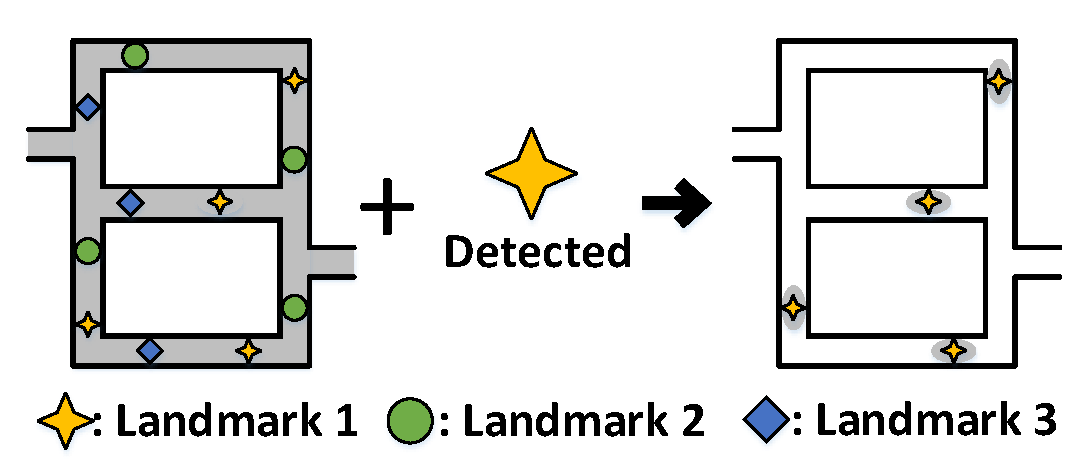
\includegraphics[width=0.8\textwidth]{apf2}\label{fig_apf_intuition2}
        \end{minipage}
        }
        \subfigure[Localization using both map constraints and detected landmarks.] {
        \begin{minipage}[b]{0.5\textwidth}
        \centering
        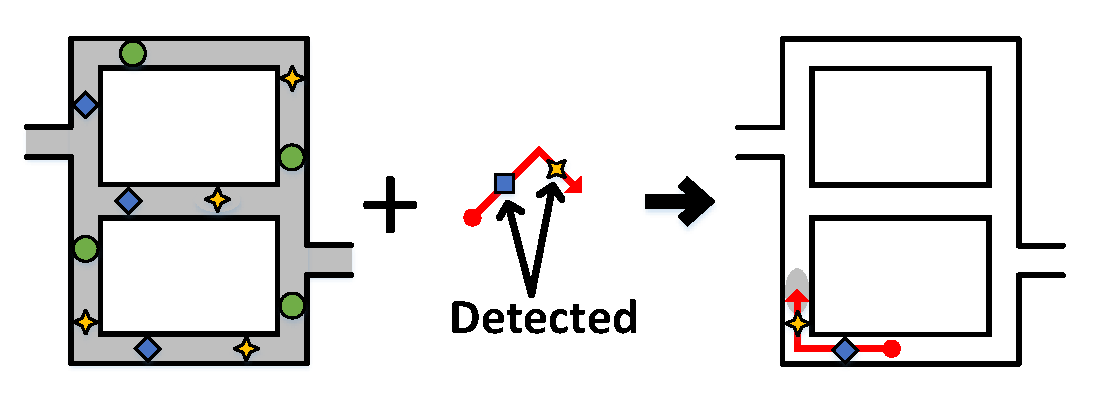
\includegraphics[width=0.8\textwidth]{apf3}\label{fig_apf_intuition3}
        \end{minipage}
        }
        \vspace{-4pt}
        \caption{Intuition of localization.
        (a) trajectories can be used for localization since only a few paths on the map could accommodate the trajectory. (b) once a landmark is detected, only a few positions marked with the same kind of landmark are possible. (c) using both map constraints and detected landmark could narrow down the uncertainty more quickly.}
        \label{fig_poster}
\end{figure}
%\section{Design Overview}\label{sec:overview}

VeLoc leverages both the floor map of the parking structure and inertial data of the driver's smartphone to track the vehicle's location. As shown in Figure~\ref{pix:overview}, Veloc consists of the following three components.
\begin{enumerate}
  \item \textbf{Pose estimation} estimates the pose, the relative orientation of the smartphone's three axes to those of the vehicle. This information is needed to transform the inertial data sensed along the phone's axes into those of the vehicle. Then the inertial data is also used to detect whether the vehicle is moving or stationary (described in Section~\ref{sec:pose}).
  \item \textbf{Landmark detection algorithms} detect three types of ground features common to parking structures, namely speed bumps, turns and slopes. These are used as calibration points so uncertainties in the vehicle's location can be greatly reduced once a landmark is detected (Section~\ref{sec:landmark}).
  \item \textbf{Realtime tracking} module employs an augmented particle filter based method to estimate the states of a vehicle (including its location, orientation, and velocity) using a probabilistic model. It exploits the constraints from detected landmarks and the floor map to reduce the uncertainty in the states so that the vehicle's location can be determined(Section~\ref{sec:tracking}).
\end{enumerate}
\begin{figure}[h]
  \centering
  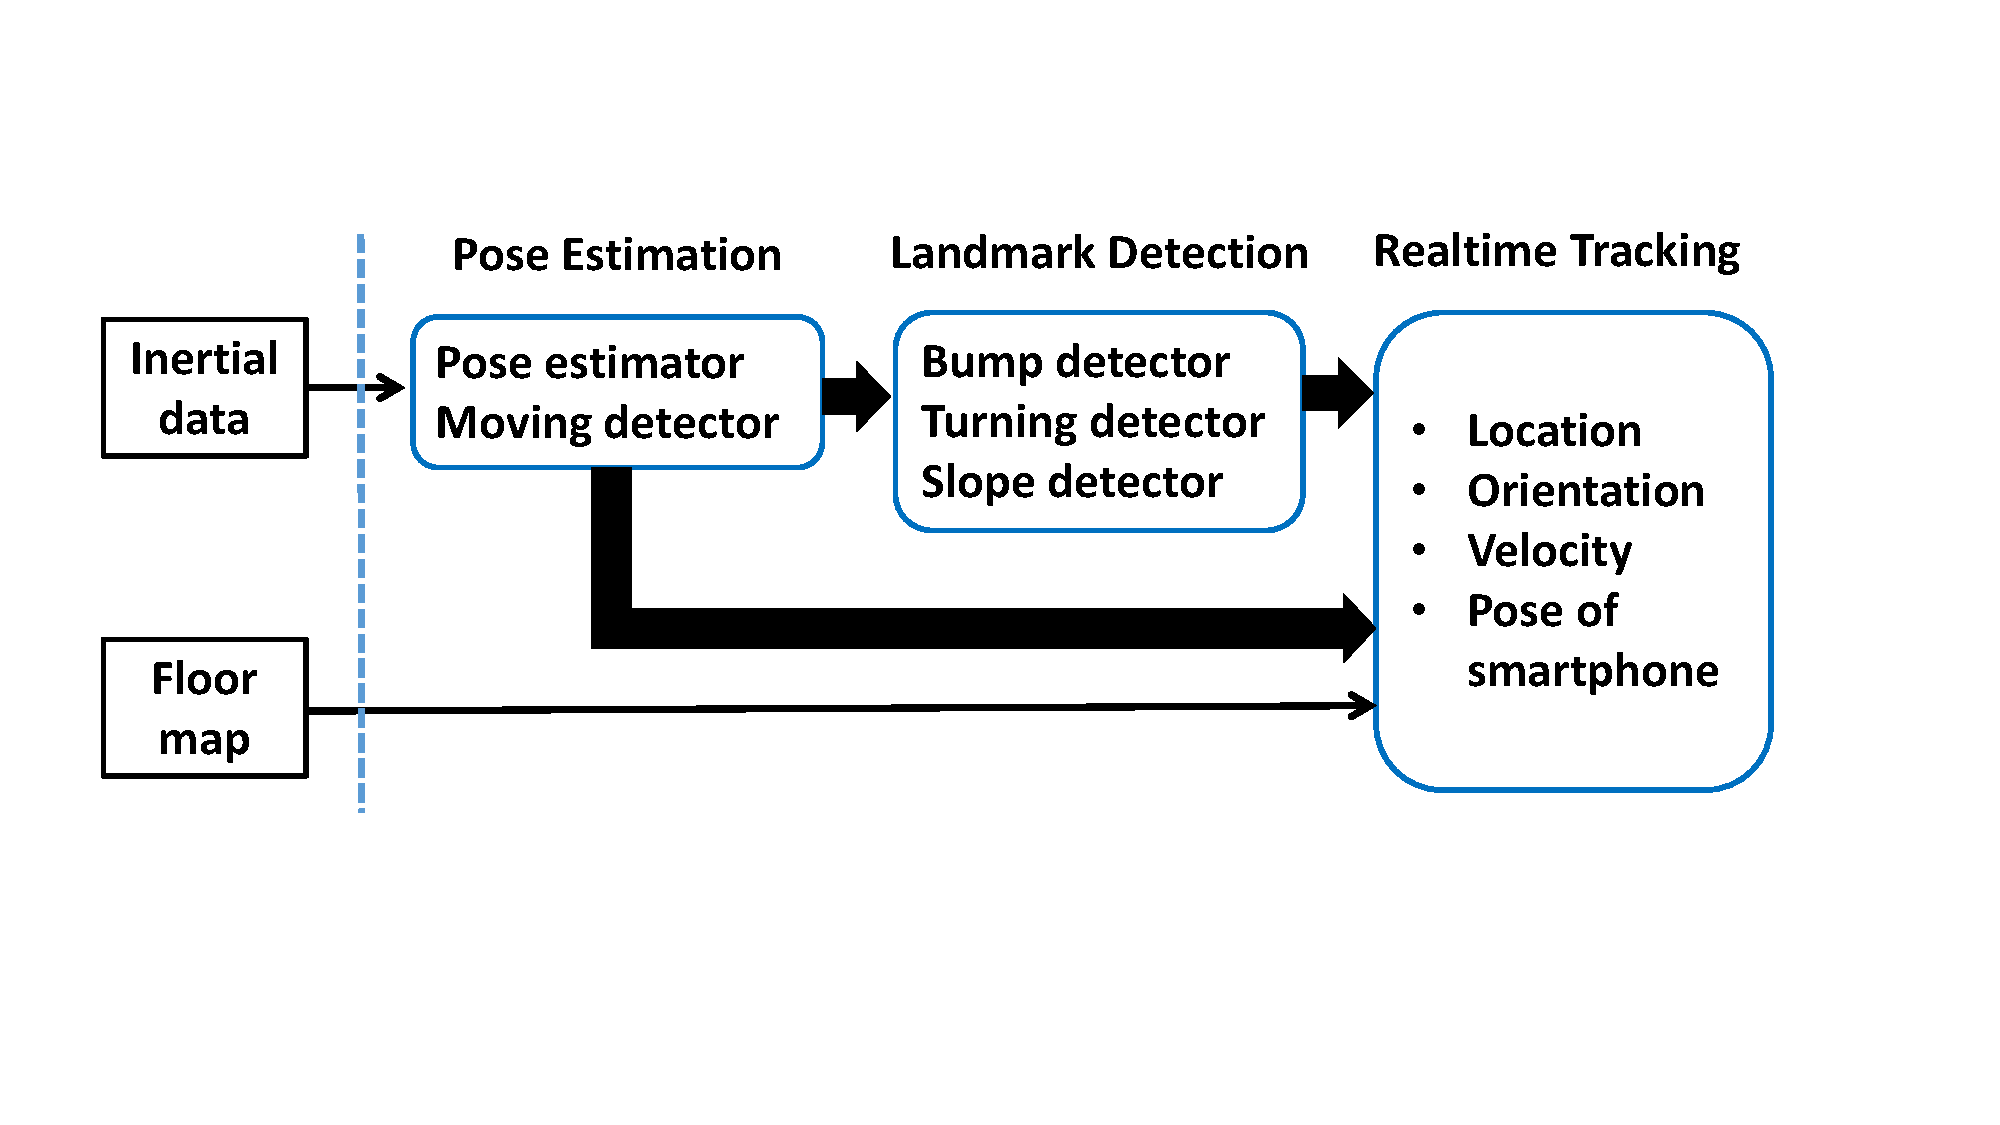
\includegraphics[width=0.5\textwidth]{overview}\\
  \caption{Three components of VeLoc. Inertial data is used to compute the smartphone's pose in the vehicle, then it is further processed to detect certain landmarks during driving, and the augmented particle filter harnesses constraints from landmark detection and the floor map for vehicle localization.}\label{pix:overview}
\end{figure}


%\section{Pose Estimation}  \label{sec:pose}
The sensor readings from a smartphone measure the physical quantity in the local coordinate system of the phone, e.g., the acceleration components along the phone's width, length and depth directions ($x', y'$ and $z'$ as shown in Figure~\ref{pix:coordinates}). Because in most cases the phone's axes are not exactly aligned with respective axes of the vehicle, a transformation is needed to derive the acceleration or attitude angles of the vehicle from those of the phone.

In this section, we describe how to estimate the directions of the vehicle's axes ($(x, y, z)$ in Figure~\ref{pix:coordinates}) in the phone's coordinate system. First, we find the direction of the vehicle's $z$ axis from the gravity, assuming that the vehicle is on a level surface. Next we detect the direction of the vehicle's $y$ axis from its acceleration and de-acceleration when moving along straight lines. After $y$ and $z$ axes are decided, the $x$ axis is determined in the phone's coordinate system as well.

%acceleration and cannot be directly used if coordinate systems of the vehicle and the smartphone do not coincide, which happens in most real world cases. As illustrated in Figure~\ref{pix:coordinates}, $(x, y, z)$ represent the coordinates of the vehicle, and $(x', y', z')$ represent the coordinates of the smartphone. In this section, we describe the method to estimate the direction of $(x, y, z)$, which we called \textit{pose} in this paper, regarding the coordinates system of the smartphone as a reference system. First, we choose the opposite direction of the gravity to be z-axis. Second, we estimate the y-axis position on the xy-plane of the vehicle during its straight driving. Finally, we derive the direction distribution of the y-axis instead of a fixed direction when the vehicle is moving forward.
\begin{figure}[h]
  \centering
  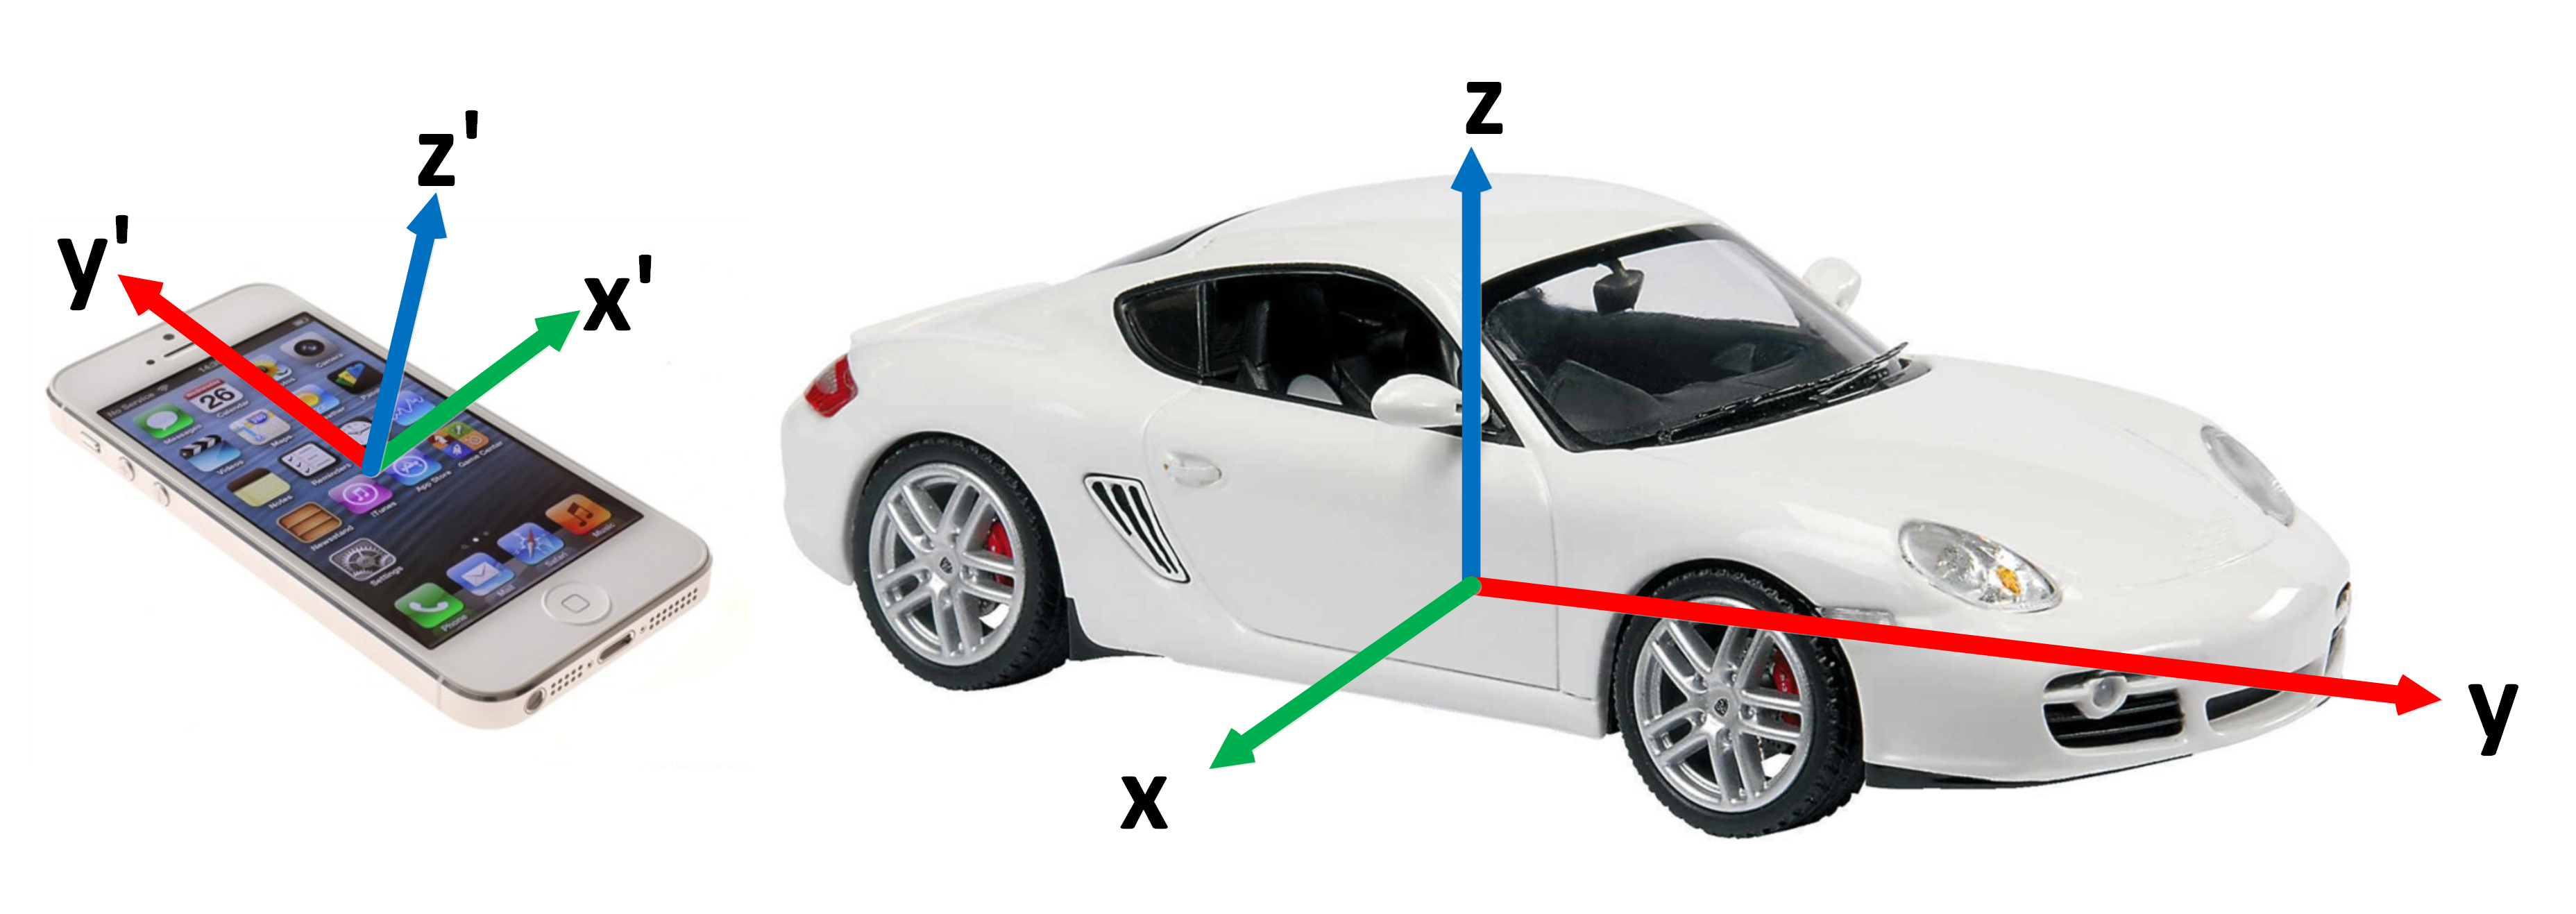
\includegraphics[width=0.5\textwidth]{coordinates}\\
  \caption{Coordinate systems of a vehicle ($x,y,z$) and a smartphone ($x',y',z'$).}\label{pix:coordinates}
\end{figure}

\subsection{Z-axis Estimation}% and Euler Angles Conversion}
The z-axis of the vehicle and the gravity are on exact opposite directions when the vehicle is on level ground. Thus we can tell the z-axis direction from that of the gravity. When the phone remains static or moves at constant speed, the only force and thus acceleration on the phone is the gravity. When the phone has other acceleration, various techniques can be used~\cite{Wang:2013_Driver_Phone_Use} to extract the components of the gravity on the phone's three axes at reasonable accuracy (e.g., iOS has an API to obtain those three components). Since vehicle movements will cause small, random disturbances on $x$ and $z$ axes acceleration even when moving along level, straight lines, we further average the extracted gravity samples within a time window. Thus such disturbances cancel out themselves on opposite directions of the same axis.

% However, the inertial sensor data of the smartphone's coordinate system may deviate from the real gravity direction because of the movement of the vehicle. To reduce this error, we averages inertial sensor data in a sliding time window and regard this as the gravity direction in the smartphone's coordinate system.

Given the z-axis direction in the phone's coordinate system, the angle the vehicle makes a turn on the $xy$ plane can be derived from the gyroscope data of the phone after a transformation. Thus we can tell whether the vehicle is moving along straight lines or making a turn.

%of the vehicle, we can derive the orientation of the smartphone on the xy-plane of the vehicle in the smartphone's coordinate system, according to the gyroscope data. This orientation is also the vehicle's orientation on its xy-plane if the smartphone is relatively static to the vehicle.

\subsection{Moving Detection}
To estimate the y-axis direction, we need to detect wether the vehicle is moving after knowing that it is not making a turn. To this end, we calculate the variance of accelerometer readings on three axes of the smartphone's coordinate system averaged within a sliding window. Theoretically, the accelerometer readings remain unchanged and the variance is zero if the vehicle is static or moving at a constant speed along a straight line. In practice, due to inevitable vibrations, small accelerations always happen and the variance cannot be zero.
%the vehicle will have vibration that can be detected by the accelerometer even it's static (xx how can it vibrate when static??).
We set a threshold and consider the vehicle static if the variance is smaller than the threshold. We find that this works very well for moving detection. Figure~\ref{pix:move} shows the normalized variance distribution during static and moving states. We can see that the overlapping portion is small compared to total areas.

\begin{figure}[h]
  \centering
  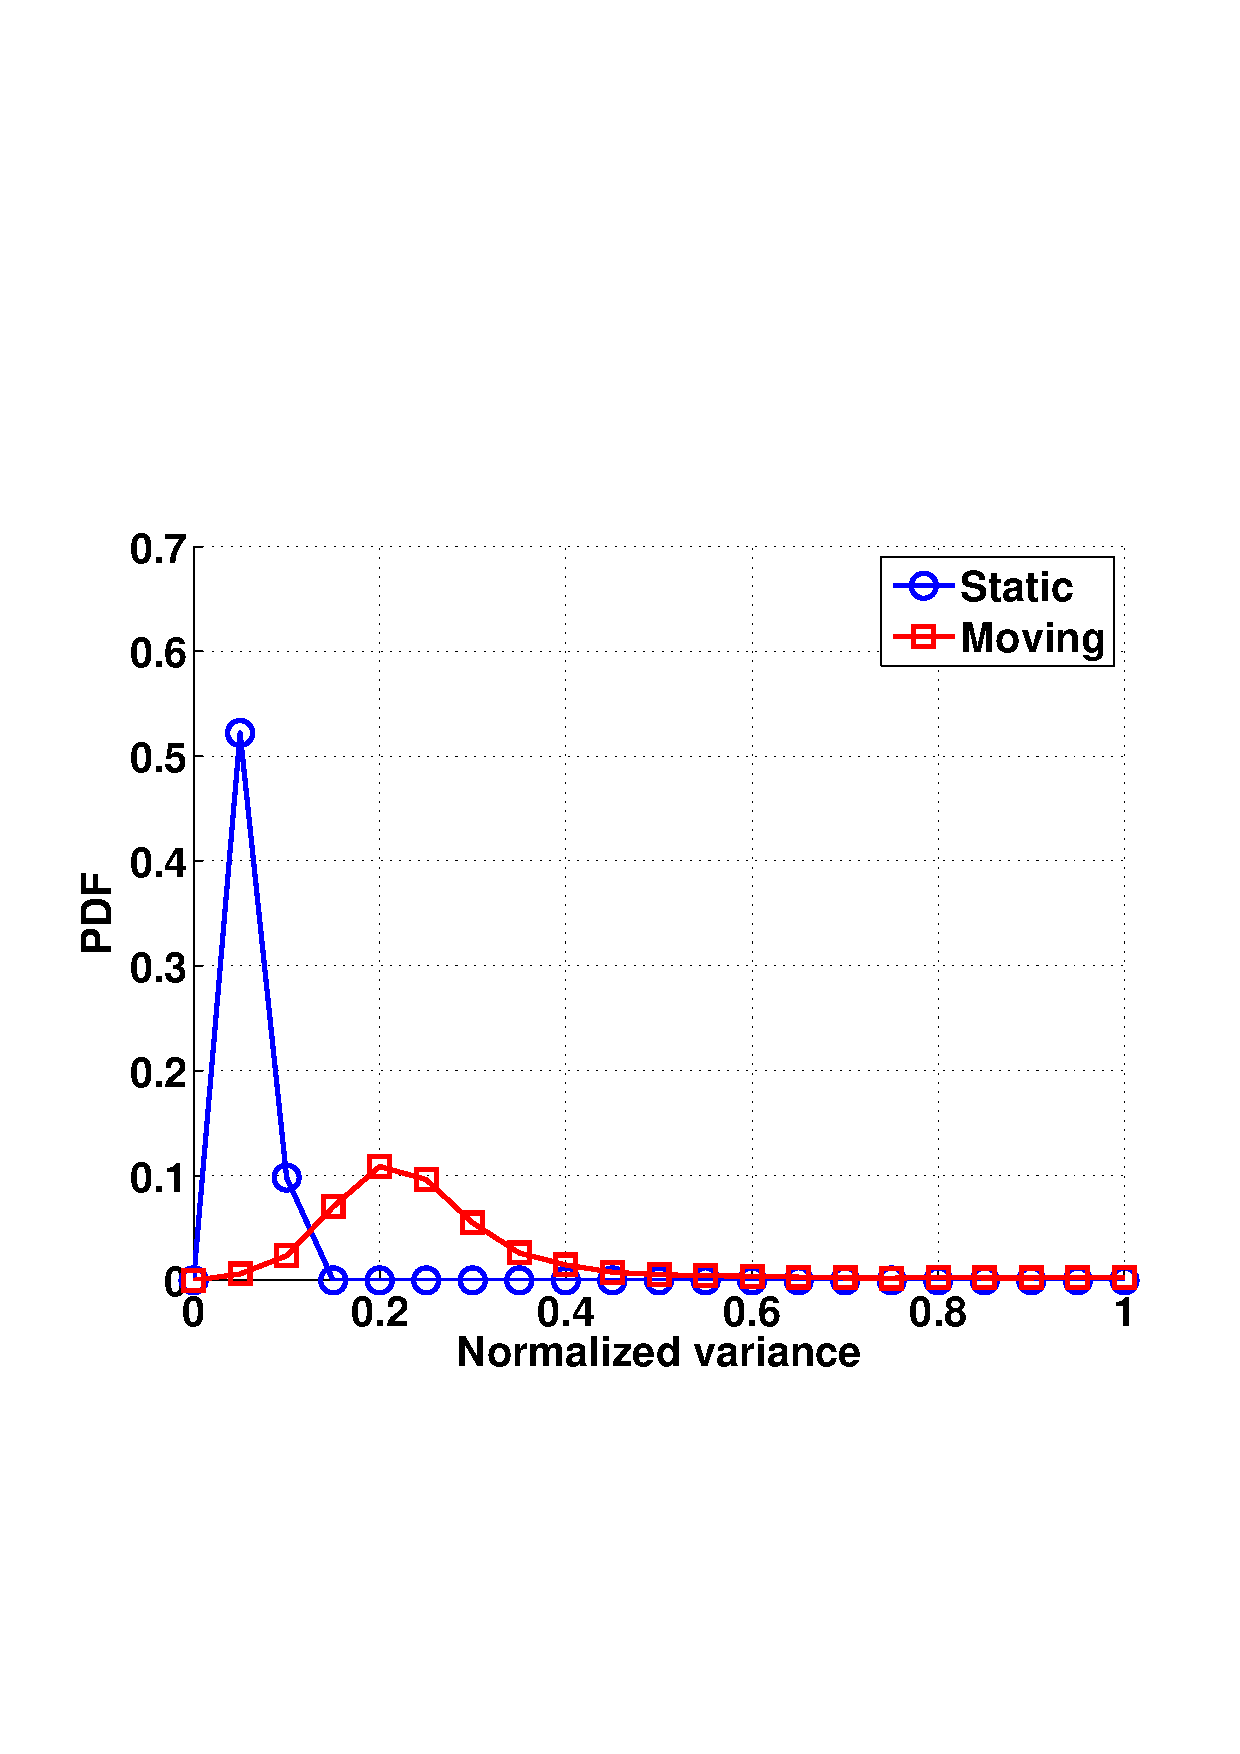
\includegraphics[width=0.35\textwidth]{move}\\
  \caption{Distribution of normalized standard deviation during static and moving states. }\label{pix:move}
\end{figure}

\subsection{Y-axis Direction Estimation} \label{subsec:pose_undirected}
Now we estimate the direction of the y-axis in the smartphone's coordinate system. During straight driving at constant speed, theoretically, the accelerometer readings are non-zero on the y-axis only (assuming gravity is removed). Thus the direction of acceleration is that of the $y$ axis in the phone's coordinate system. In practice, there are some noise on the x-axis because roads cannot be perfectly smooth.

Suppose that the direction of acceleration on the $xy$ plane is represented by a unit vector ${(cos\theta, sin\theta)}$ on the xy-plane of the vehicle. Given a set of accelerometer samples, we first project them onto the $xy$-plane of the vehicle. This can be done because the $z$ axis' direction is known. Denote the projected results ${(x_i,y_i), i = 1,...,k}$. We want to find the $\theta$ such that the total deviation of each of them from the true $y$ axis direction is minimized:
\begin{eqnarray}
&&\sum_{i=1}^{k}(x_icos\theta + y_icos\theta)^2\\
&=&asin2\theta + bcos2\theta + c\\
&=&\sqrt{a^2+b^2}sin(2\theta + \gamma) + c
\end{eqnarray}
where ${a=\sum_{i=1}^{k}x_i y_i}$,${b=\sum_{i=1}^{k}\frac{x_i^2-y_i^2}{2}}$,${c=\sum_{i=1}^{k}\frac{x_i^2+y_i^2}{2}}$,${tan\gamma=\frac{b}{a}}$.

This equation has a closed-formed solution:
\begin{equation}
\theta_1 = \frac{1}{4}\pi -  \frac{\gamma}{2}~~~~\theta_2 = \frac{5}{4}\pi - \frac{\gamma}{2}
\end{equation}
In the solution, we can see that there are two optimal solutions to ${\theta}$, representing the forward and backward directions of the vehicle, denoted by $\theta_1$ and $\theta_2$. Next we decide which is the true direction of the y-axis of the vehicle (i.e., the forward direction).

\subsection{Forward Direction Estimation} \label{subsec:pose_directed}
%(xx this part is very difficult to follow even after my revision. Someone familiar with the process should do another pass!!)

First we suppose that $\theta_1$ is the correct direction. Then we can get the estimated $(x, y, z)$ directions in the smartphone's coordinate system and project acceleromater readings to this coordinate system of the vehicle. In a short time period when the vehicle starts moving from static, there should be more positive acceleration on the y-axis direction.

We use a sliding time window starting at the beginning of the trace. Once we detect that the vehicle starts moving in this time window, we calculate the proportion of positive accelerometer readings within this time window such as:
\begin{equation}
\rho = \frac{1}{k}\sum_{i=1}^{k}y_i^3
\end{equation}
We use cubic form rather than linear form to better filter small noises caused by vibration of the vehicle, and focus on the real accelerometer readings caused by the acceleration of the vehicle.

% representing the forward and backward directions of the vehicle, denoted by $\theta_1$ and $\theta_2$.

However, this value is insufficient to determine whether $\theta_1$ or $\theta_2$ is the correct direction. Then, we put this value into sigmoid function and derive a probability of how $\theta_1$ likely equals $\theta$:
\begin{equation}
p(\theta=\theta_1)=\frac{1}{1+e^{-\rho}}
\end{equation}
The particle filter (in Section~\ref{sec:tracking}) then uses this probability as a prior to accurately converge on the correct direction---$\theta_1$ or $\theta_2$. This method helps narrow down the uncertainty caused by two opposite directions. % $\theta_1$ and $\theta_2$.






%\section{Landmark Detection}\label{sec:landmark}

%Special road conditions, which we call landmarks, cause particular pattern in inertial sensor data.
Landmarks along a road in certain environments are highly likely to cause distinguishable patterns in the observed inertial sensor data when a vehicle passes over them. Typical landmarks in a parking structure include bumps, turns, and slopes. In this section, we present three robust algorithms for detecting these three types of landmarks using inertial sensor data.

\subsection{Bump Detection}
Bumps are used to limit the vehicle speed inside parking lots for the sake of safety. When a vehicle pass over a bump, it causes a jolting that generates a detectable pattern in the inertial sensor data. Note that other landmarks such as drainage outlets or joint part of fire shutters, may also cause similar jolting patterns as bumps and thus are categorized as bumps as well in this paper.

\textbf{Acceleration-based detection}. When a vehicle passes over a bump, jitters occur in the signals of both accelerometer and gyroscope sensors of a smartphone inside the vehicle. Acceleration along the z-axis (the vertical direction) can best characterize such jitters.
%Moreover, gyroscope signals along x- or y-axis are also helpful for detecting the road anomaly as these signals are always near-zero unless there is some road anomaly that causes vibrations.

Some previous work \cite{Eriksson:The_Pothole_Patrol} calculate the standard deviation of the z-axis acceleration, and use a pre-determined threshold to detect bump-passing. Figure~\ref{fig_bump}(a) shows the acceleration on the z-axis for a car driving over four bumps along a straight road, and the standard deviation is shown in Figure~\ref{fig_bump}(b). The first jitter at the 4th~second is from a sudden change of the phone's pose, which is less significant than other four caused by the bumps.

However, due to the variation of parking lots structures, vehicle models and driving styles, it is difficult to find a universal threshold that fits all cases. Moreover, occasional phone pose changes during driving may also cause false alarm (e.g, the one at the 4th~second in Figure \ref{fig_bump}~(b)).

% (a)
% ���ĸ�peak �ú�ɫȦ �����
% �����һ�� peak �� ���� jitters �ü�ͷָ������һ�� front wheel��һ�� rear wheel


% (b) ��ͼ�У��Ե��ĸ� vibration ���ʲô�� inter-jitter period

\begin{figure}[t]
      \centering
      \vspace{-2pt}
        \subfigure[Acceleration along the z-axis with four jitters.] {
        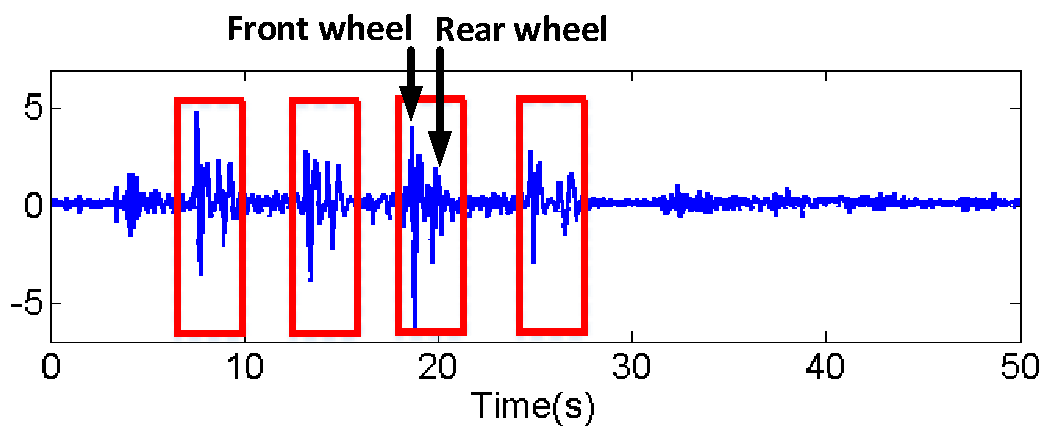
\includegraphics[scale=0.4]{detect_1}\label{detect_1}
        }
        \subfigure[Standard deviation with four high peaks] {
        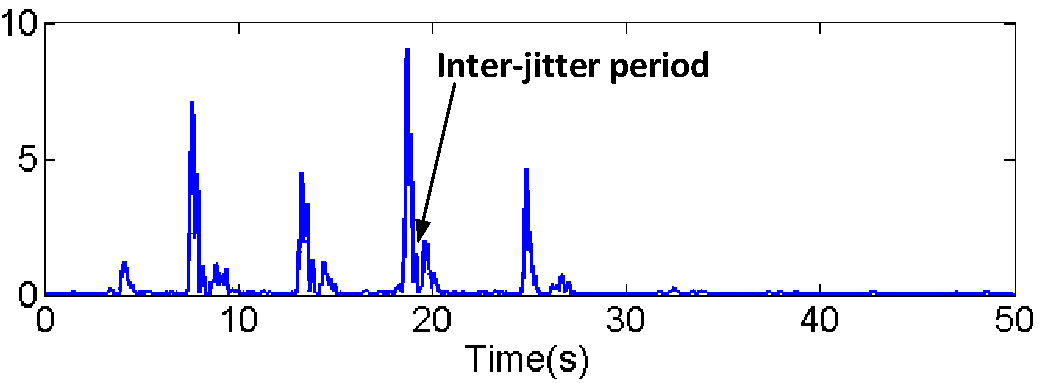
\includegraphics[scale=0.4]{detect_2}\label{detect_2}
        }
        \subfigure[Convoluted standard deviation with four distinguishable peaks] {
        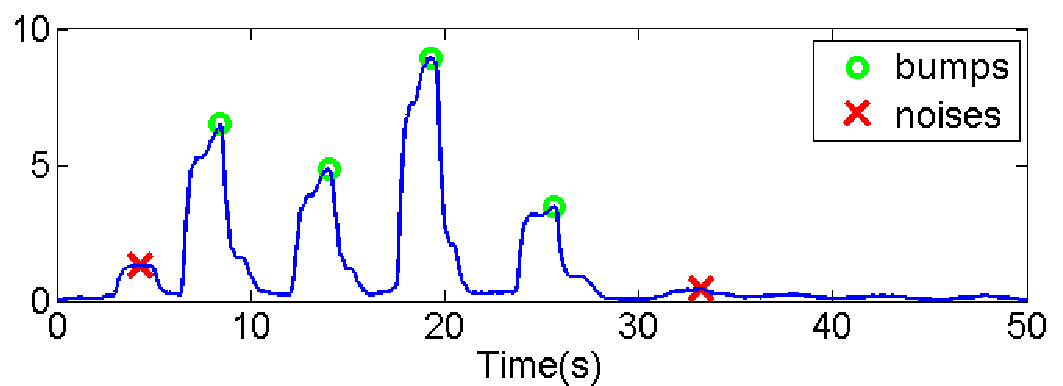
\includegraphics[scale=0.4]{detect_3}\label{detect_3}
        }
        \caption{Bump detections: (a) four jitters (circled ones in the figure) in the acceleration on the z-axis; (b) four high peaks in the standard deviation of the z-axis acceleration; (c) four distinguishable peaks after applying convolution to the standard deviation with a Gaussian filter, where green (or red) markers indicate the local maximums for detected bumps (or false alarms).}\label{fig_bump}
\end{figure}

\textbf{Proposed bump detection algorithm}. We propose a robust bump detection algorithm that is less sensitive to the choice of the threshold and occasional pose changes of the phone.

We observe that when driving straight, each bump can incur two consecutive car jolts when its front wheels pass over a bump followed by rear ones. Note that the first jolt usually is more significant than the second as the phone is often placed in the front of a car, and it is also because that the vehicle's speed usually has been reduced when the front wheels pass over the bump. Or a bump may cause four jitters at a turning corner because each of wheels' pass over the bump at different times. These consecutive jitters lead to two or four peaks in the standard deviation of the z-axis acceleration. We smooth the standard deviation curve by convolving it with a Gaussian filter. The two jitters caused by a bump in Figure~\ref{fig_bump}(b) is merged into a single distinguishable peak in Figure~\ref{fig_bump}(c). The time stamp of the peak is the time when the center of the vehicle is passing over the bump. After the convolution, it is much easier to distinguish jolts caused by bumps from those incurred by sudden phone pose changes, because the latter does not have subsequent followers.

%, and the gap between the peaks is very short (namely ``jitter gap'') The middle time point of such consecutive jitters and inter-jitter periods is a good estimate of the time point when the center of a vehicle crosses the bump. Instead of observing the magnitude of jitters or vibrations, we use the estimated time point when the center of a vehicle crosses the bump as a central decision statistic.
% exact time at which the center of the vehicle have the same 2D coordinates with the bump.

%To estimate the middle of consecutive inter-jitter periods,

% bump is a longer process then vibrating caused by sudden pose change. A threshold is used to decide whether those candidates are real bumps.


%We define $E(s,t)$, the \emph{Energy} of a signal $s(t)$ at time $t$ as standard deviation of $s(t)$ in the time window [$t-\delta t$,$t+\delta t$]
%where $\delta t$ is the window size. The feature used for road anomaly detection is defined as follows:
%\begin{equation} F_1(t):=E(acc_z,t)+\frac{E(gyr_x,t)}{b}+\frac{E(gyr_y,t)}{b}\end{equation}
%$b$ is used to balance the difference in scale between two kinds of data. In VeLoc, we set $b=(0.1)^2=0.01$.\\


%\begin{figure}
%  \centering
%  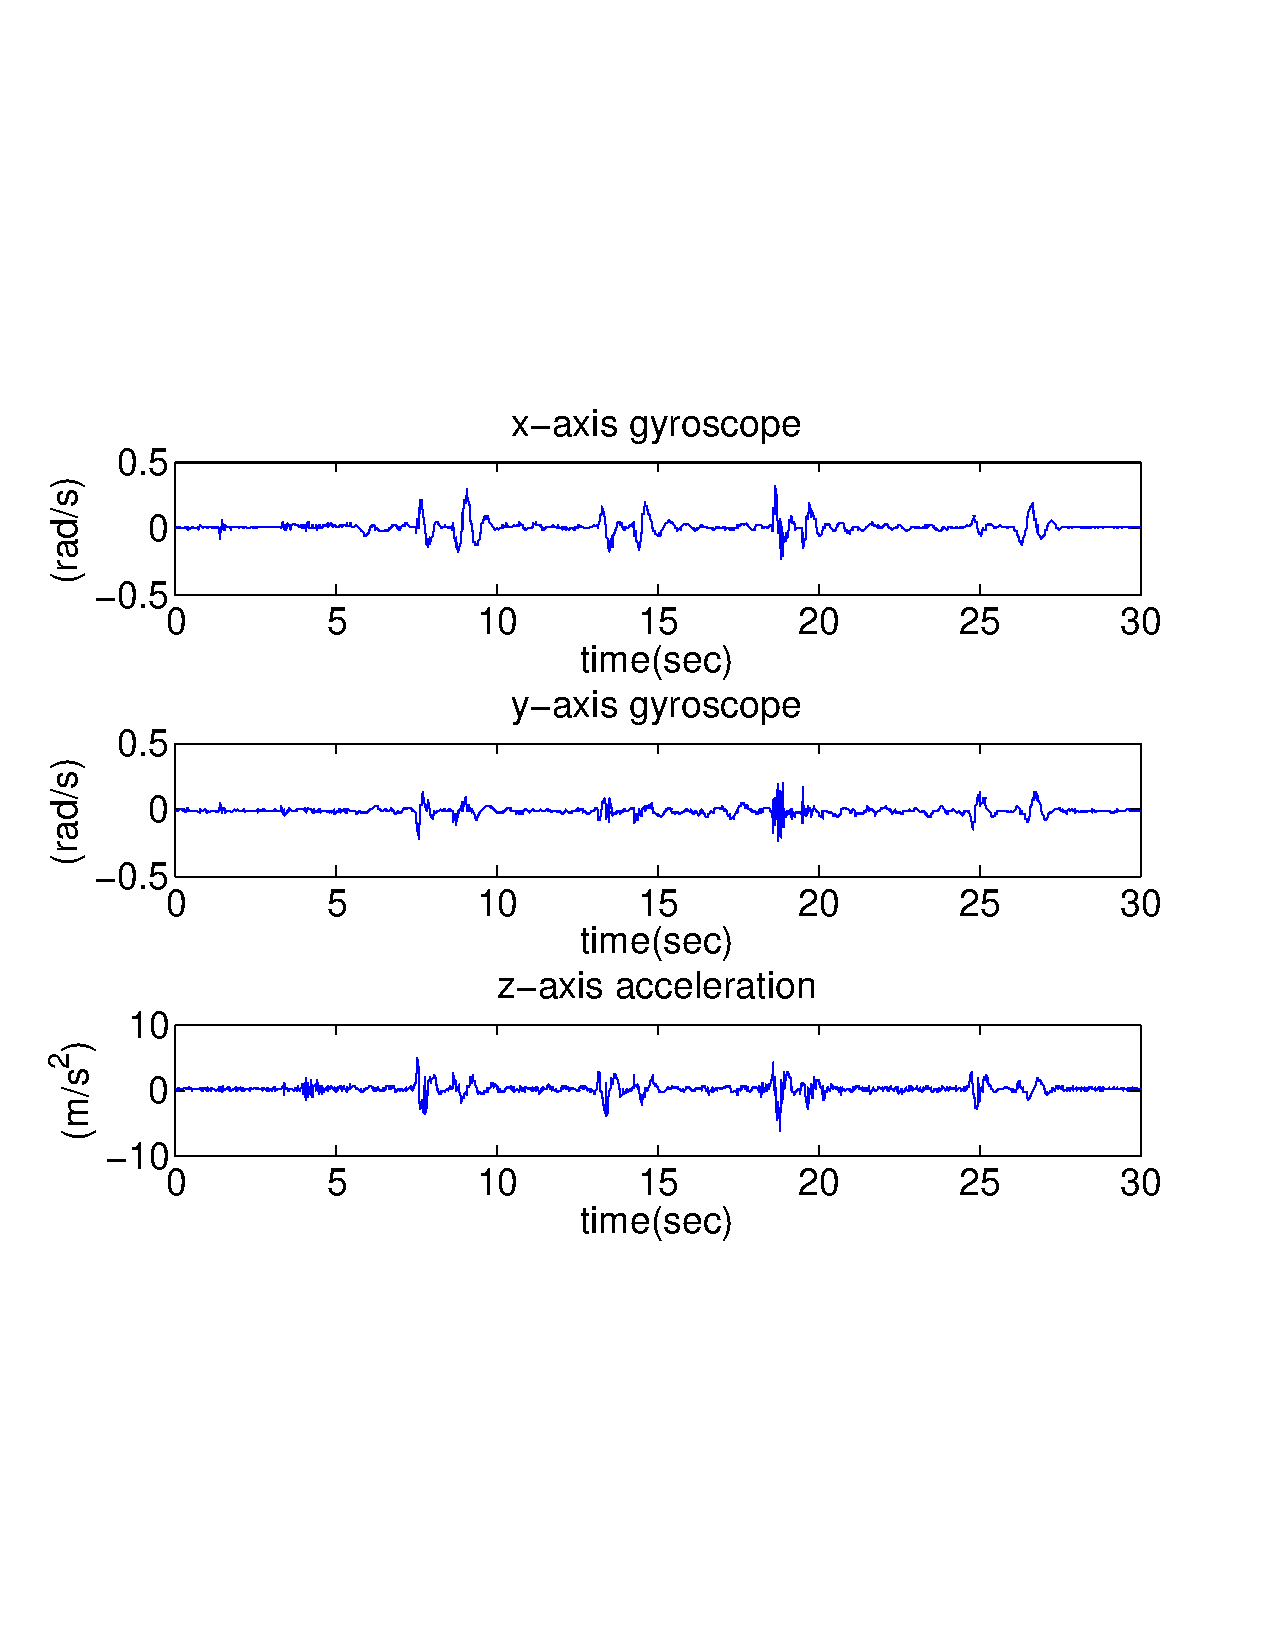
\includegraphics[width=0.5\textwidth]{raw_data}\\
%  \caption{sdf}
%\end{figure}


%There are some existing approaches based on the acceleration on z-axis to detect bumps on the road\cite{}.
%One idea is to calculate standard deviation(shown in Figure X) and use a threshold to detect the bumps.
%However, different parking lots, different vehicles and different driving style make it hard to find a threshold suitable for all cases.
%Standard deviation for three driving cases by the same driver in three different parking lots depicted in Figure X shows the difficulty of threshold selection.
%Additionally, occasional pose change during the driving also lead to high deviation in acceleration on z-axis.
%For instance, during the drive shown in Figure X, the sudden start at around 5s change the pose of phone, thus, standard deviation is relatively high to be confused with bumps.
%We propose a bump detection algorithm unaffected by threshold and robust to occasional pose change.
%The intuition is that there are two jittering corresponding to the front pair of tires and rear pair of tires when a vehicle come across to a bump.

\subsection{Turn and Slope detection}
Both turns and slopes can be detected by gyroscope signals when rotational velocities are measured: horizontal turns result in rotational velocity along the z-axis as shown in Figure \ref{fig_turn_slope}(a)(b), and slopes lead to rotational velocity along the x-axis as shown in Figure \ref{fig_turn_slope}(c)(d).
Based on this observation, VeLoc calculates the accumulated rotation angle as the detection statistic,
\begin{equation}
C(t;{\bf s},k) = | \sum_{\tau=t-k}^t{{\bf s}(\tau)} |,
\end{equation}
where ${\bf s}(\tau)$ is the gyroscope reading at time $\tau$ of an axis, and $k$ defines the size of the data collection window. The magnitude of $C$ depends on the angle that the vehicle turns.
\begin{itemize}
  \item \textbf{A turn} is detected at time $t$ if and only if
\begin{equation} C(t;{\bf s}_z,k)> \frac{\pi}{6} \end{equation}
where ${\bf s}_z$ is the gyroscope signal along the z-axis.
  \item \textbf{A slope} is detected at time $t$ if and only if
\begin{equation} C(t;{\bf s}_x,k)> \frac{\pi}{18}, \end{equation}
where ${\bf s}_x$ is the gyroscope signal along the x-axis. Both the thresholds are chosen empirically.
\end{itemize}


\begin{figure}[t]
      \centering
      \vspace{-2pt}
        \subfigure[Left turn] {
        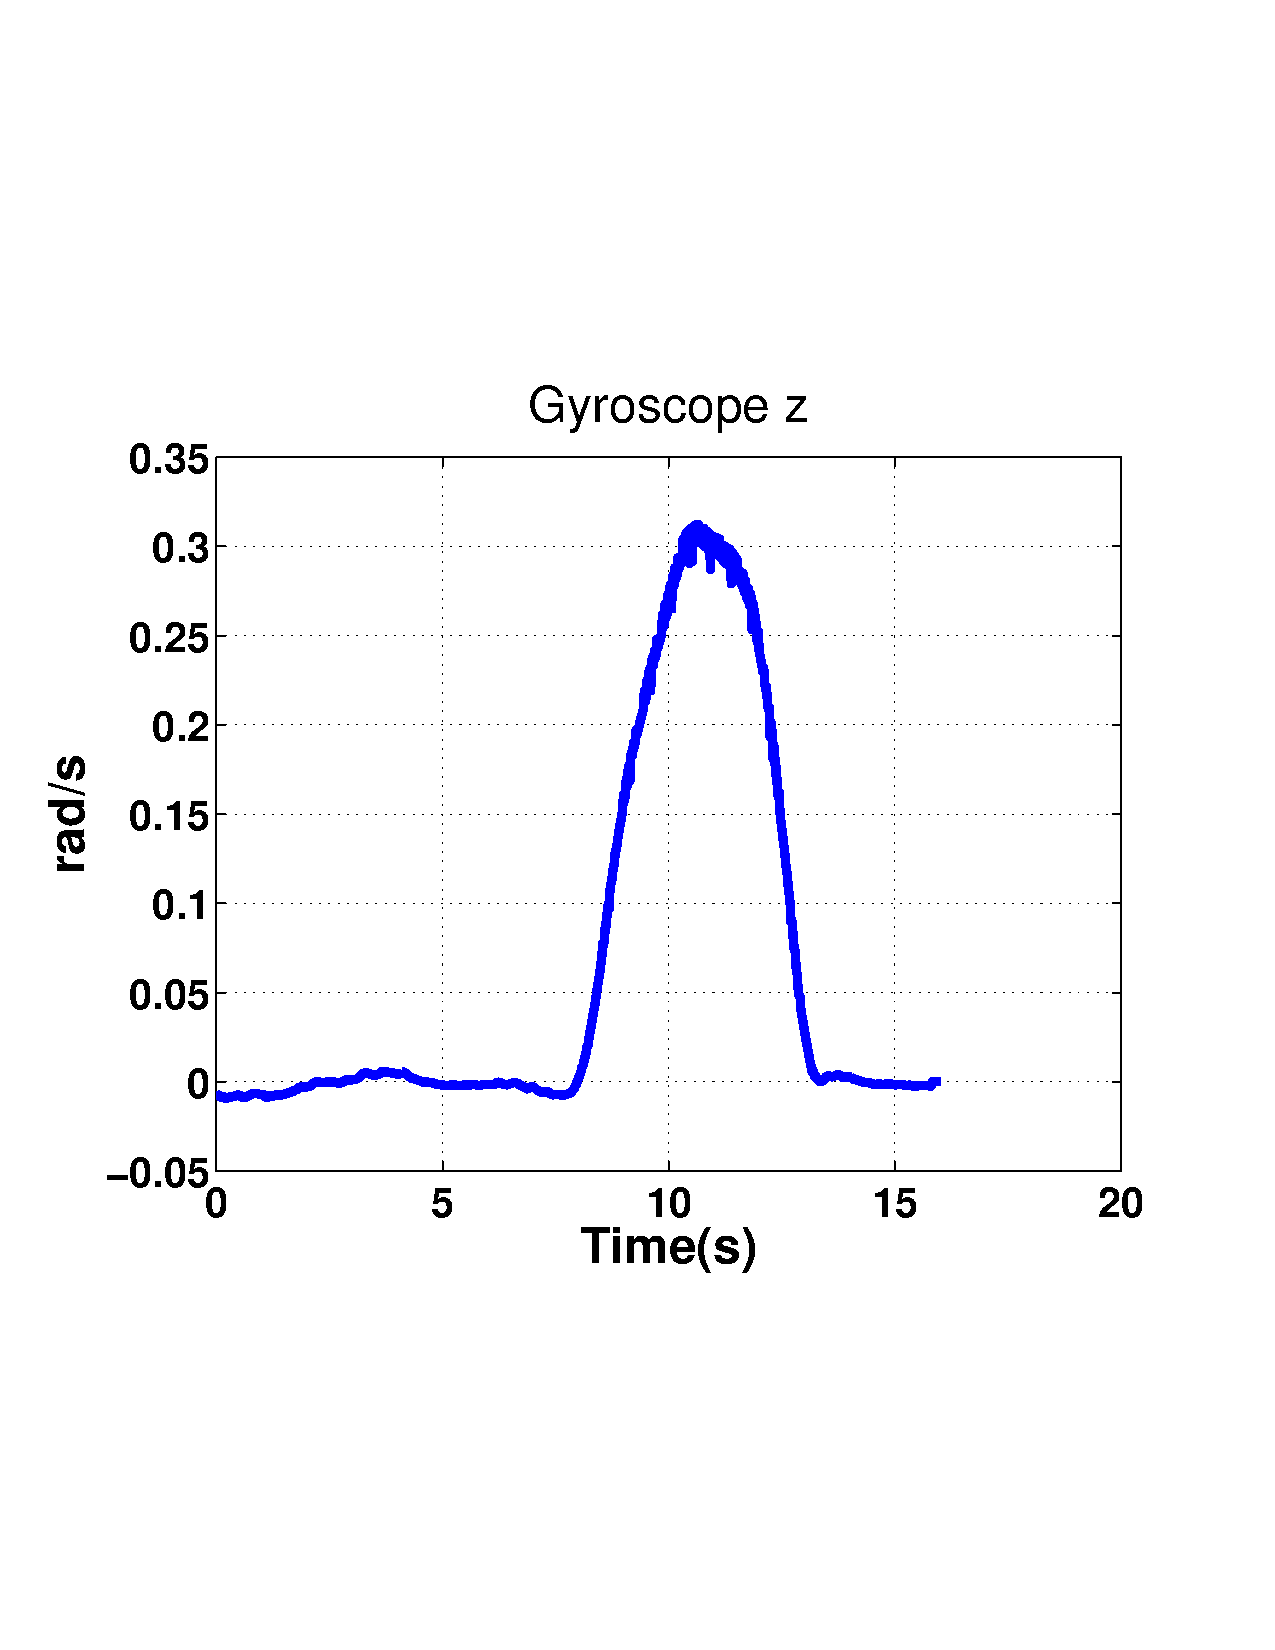
\includegraphics[width=1.55in]{left_turn}\label{left_turn}
        }
        \subfigure[Right turn] {
        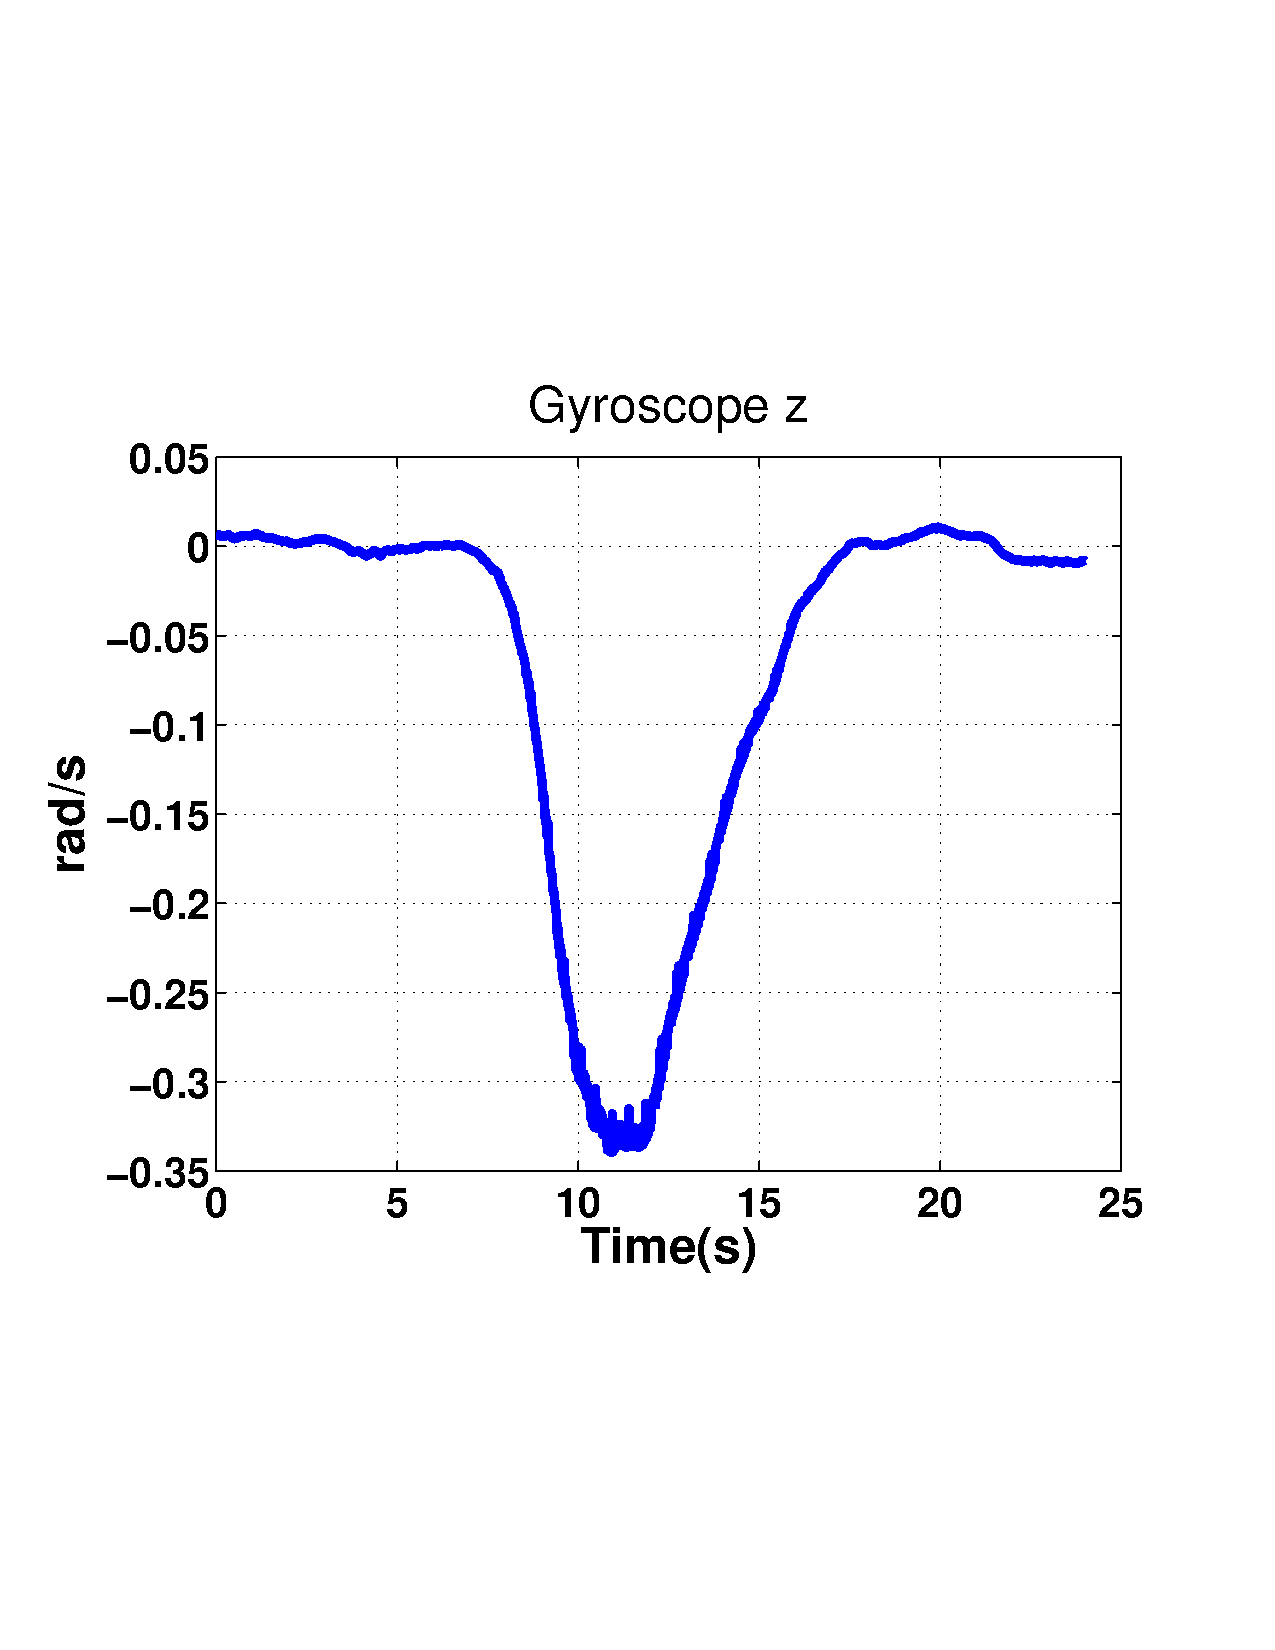
\includegraphics[width=1.55in]{right_turn}\label{right_turn}
        }
        \subfigure[Up slope] {
        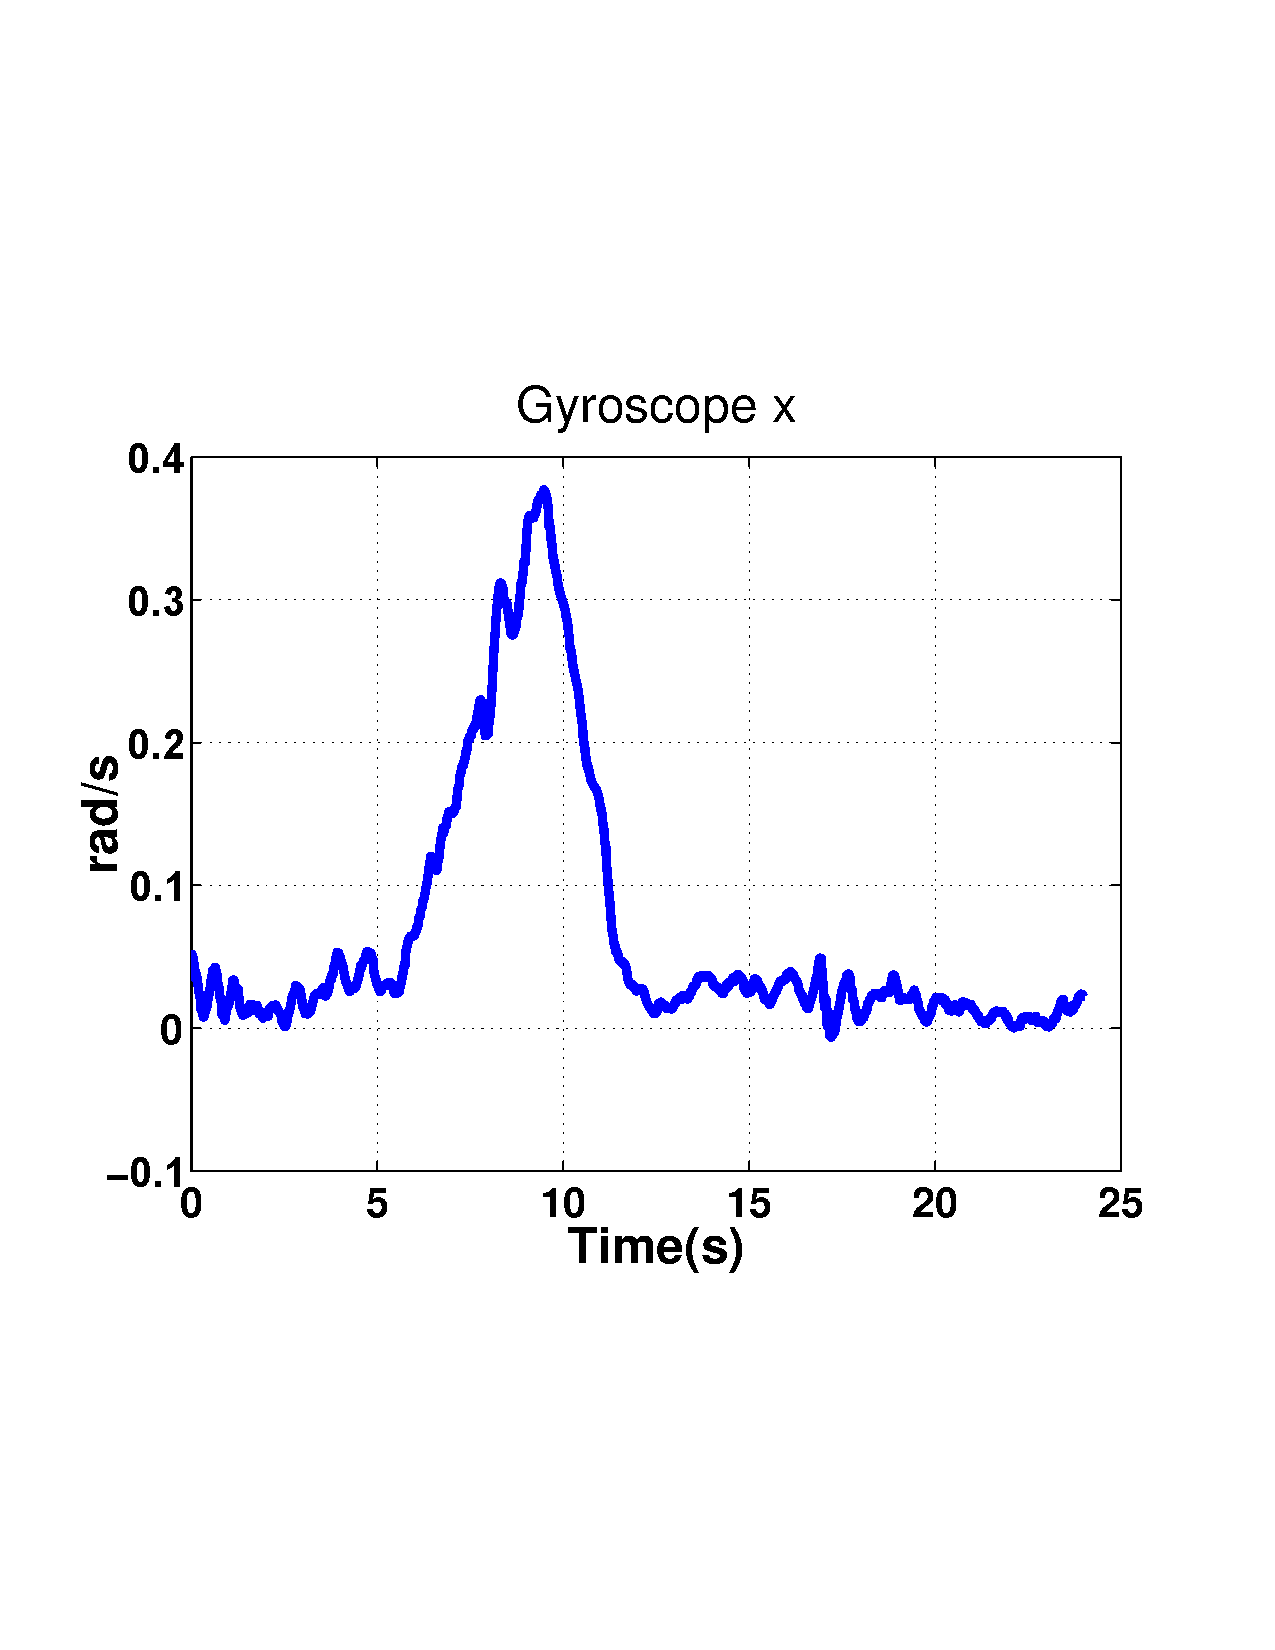
\includegraphics[width=1.55in]{up_turn}\label{up_turn}
        }
        \subfigure[Down slope ] {
        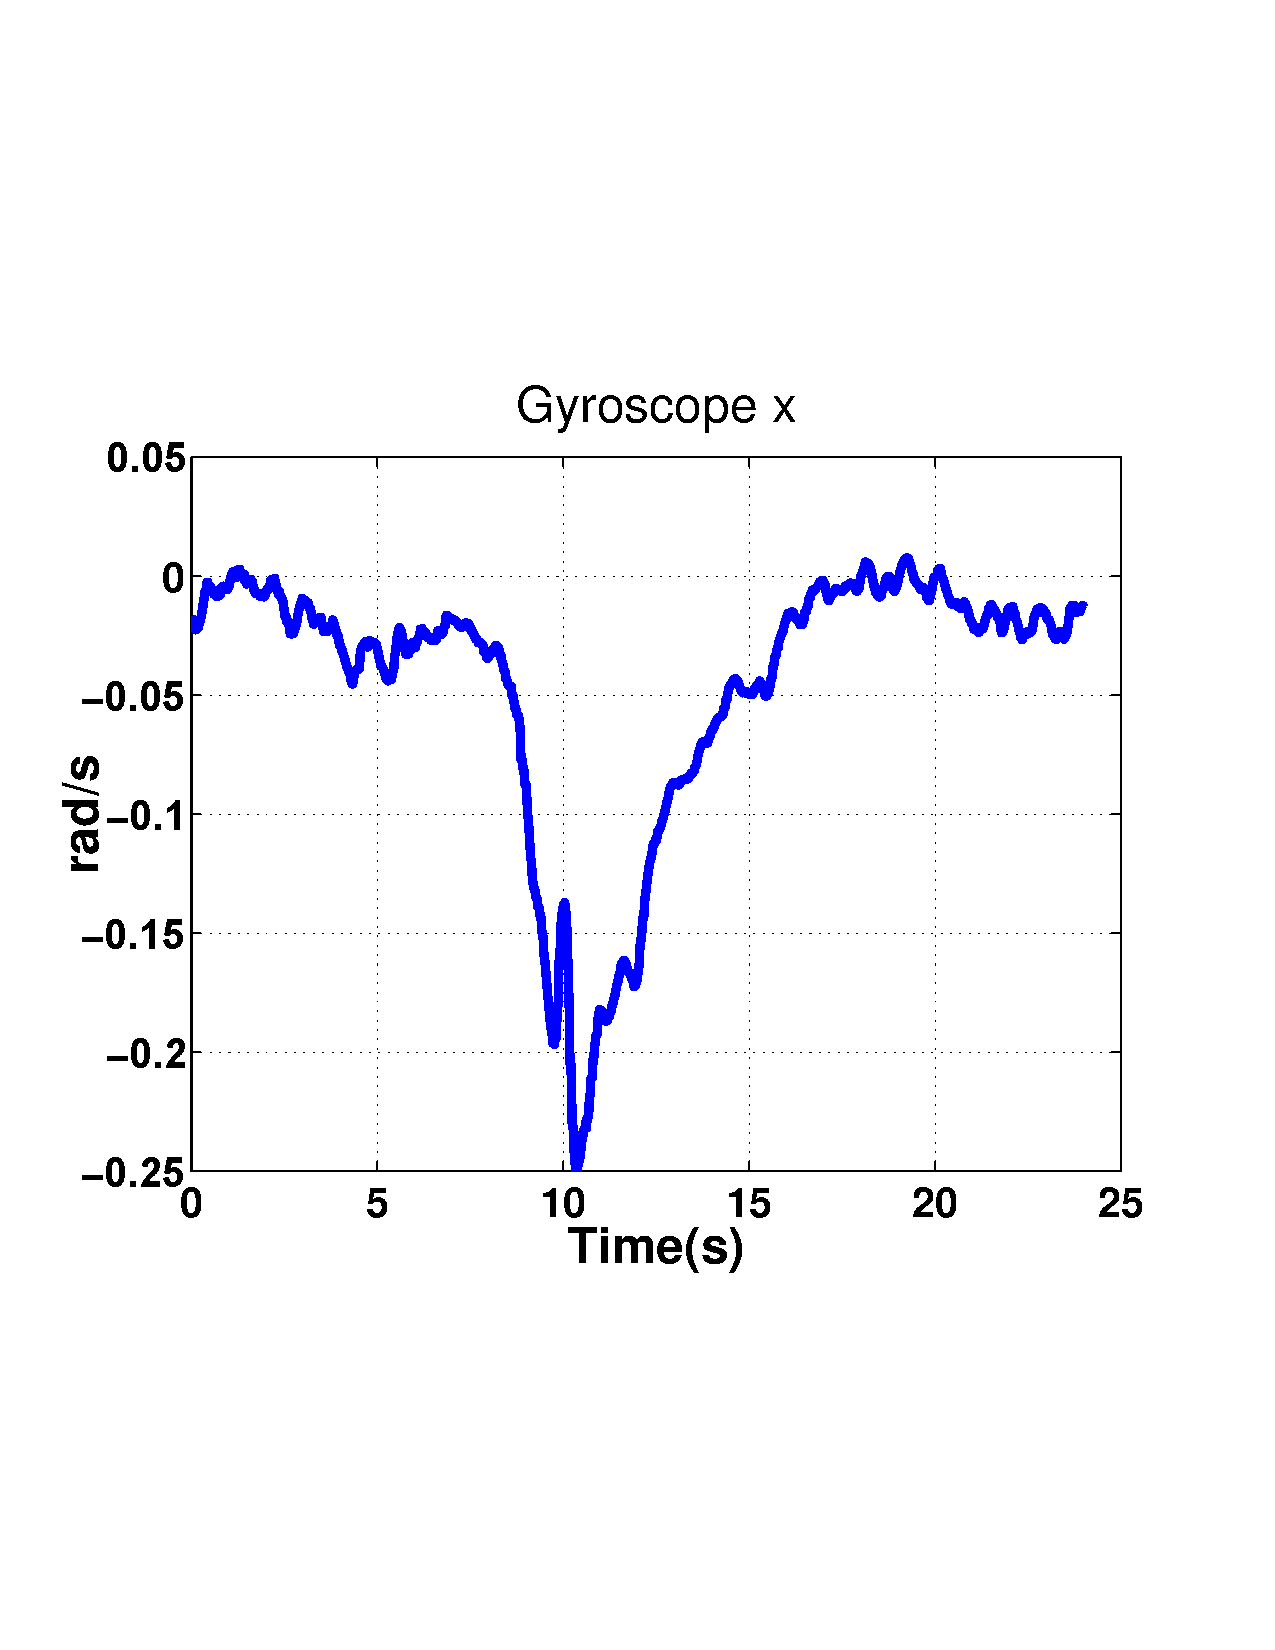
\includegraphics[width=1.55in]{down_turn}\label{down_turn}
        }
        \vspace{4pt}
        \caption{Inertial sensing data used for turn and slope detection. (a)(b) show turns using gyroscope signal along the z-axis. (c)(d) show slopes using gyroscope signal along the x-axis.}
        \label{fig_turn_slope}
\end{figure}

%During the example drive, feature $F_3$ calculated for turning detection is shown in Figure \ref{fig_features}(c) while feature $F_4$ calculated for slope detection is shown in Figure \ref{fig_features}(d).
%Note there are four responses corresponding to four turnings shown in the Figure \ref{fig_route}. The vehicle turns around key points C(22s), D(33s), E(40s), F(44s). Since there is no slope, feature $F_4$ always has a very small response.

%The magnitude of the response depends on the degree of the angle that the vehicle turns. For instance, the vehicle do not take a full 90-degree turn at the two consecutive turnings at E, F which correspond to two lower peaks.













\iffalse
The intuition behind our algorithm is that both anomalous road conditions and whether the vehicle is moving are reflected in features of the acceleration data. For the sake of clarity, we will illustrate this part with an example scenario. Figure \ref{fig_route} shows the map of an underground parking lot with route drawn on it. 7 key points, i.e. A to G, are demonstrated with time stamps. Figure \ref{fig_raw} shows the sensor data while the vehicle is moving along the route.

%\begin{figure}[htbp]
%\centering
%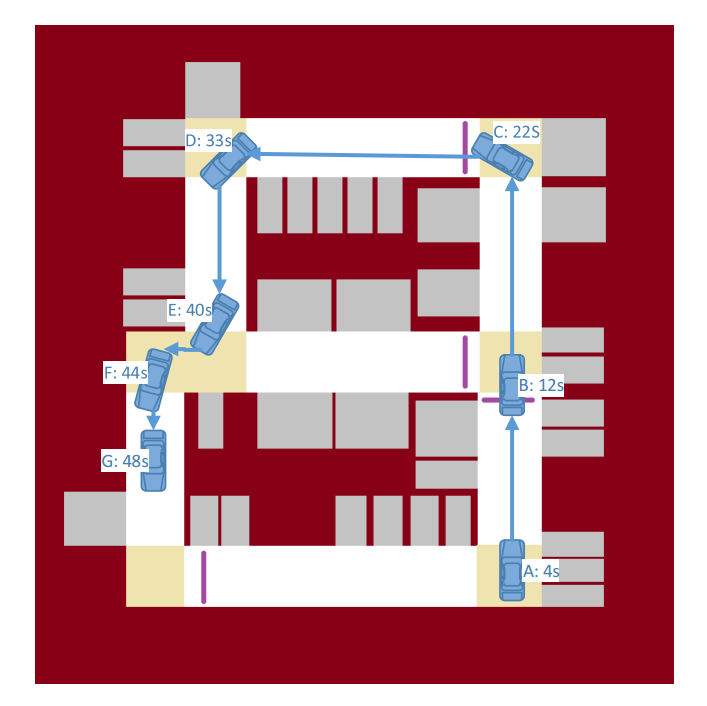
\includegraphics[scale=0.35]{route.png}
%\caption{Map of the example scenario shown with route. 7 key points are demonstrated with time stamps. The vehicle starts at A and stopped at G. The timer starts before the vehicle starts and it's time is recorded at every key point.}\label{fig_route}
%\end{figure}


%\begin{figure}[htbp]
%\centering
%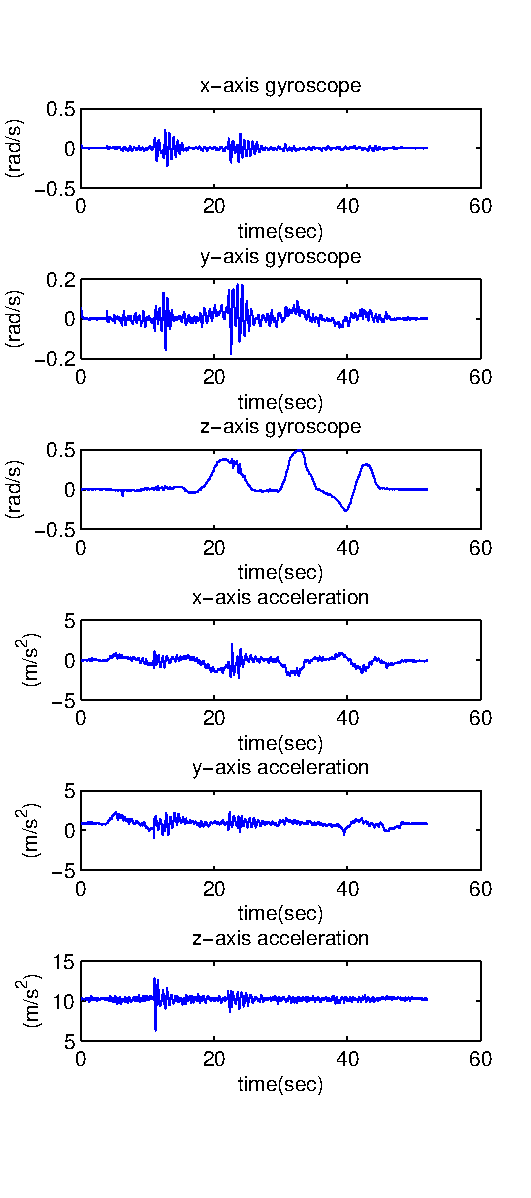
\includegraphics[scale=.7]{raw}
%\caption{Sensor data recorded during the example drive.}\label{fig_raw}
%\end{figure}

We will discuss the features used in different tasks first and then use a machine learning method to optimize all the parameters in our model.

%\begin{figure}[hbp]
%\centering
%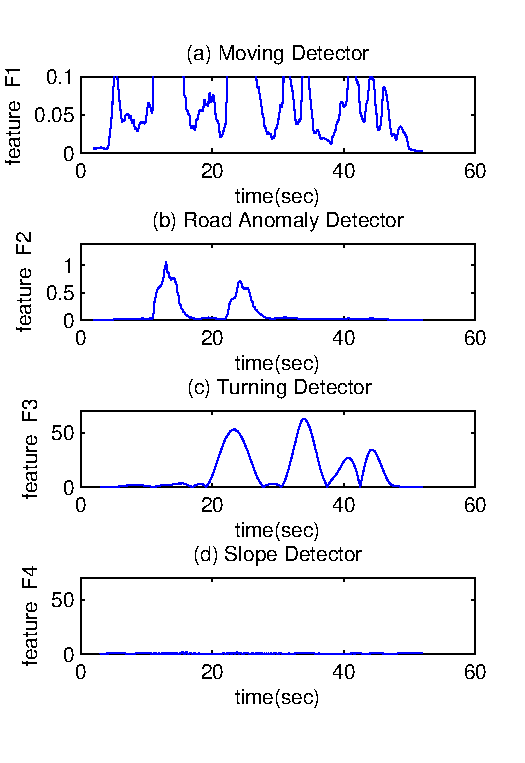
\includegraphics[scale=.7]{features}
%\caption{Features calculated for different detectors.}\label{fig_features}
%\end{figure}

\iffalse
\subsubsection{Moving Detection}
We can distinguish immobile from moving with constant speed, in principle, if the floor is absolutely flat. However, in practice, the floor of the parking lot cannot be that flat at all which cause vibration on sensor data while the vehicle is moving. Based on this intuition, VeLoc calculate the following feature of a signal $s(t)$:
\begin{equation} E(s,t) = \int_{t-\delta}^t{s(x)^2}dx \end{equation}
and discrete version with standardization:
\begin{equation} E(s,t) = \sum_{i=t-k+1}^t{s(i)^2} - \frac{1}{k}\{\sum_{i=t-k+1}^t{s(i)}\}^2 \end{equation}
where both $\delta$ and $k$ describe the window size.In our implementation, $k=100$ corresponding to $\delta=2s$ since sensor data is collected every $0.02s$ in VeLoc.\\

Feature used in moving detection is defined as:
\begin{equation} F_1(t):=w_{11}E(acc_x,t)+w_{12}E(acc_y,t)\\+w_{13}E(acc_z,t)\end{equation}
where $w_{11},w_{12},w_{13}$ are weights summing up to 1.\\

Vehicle is regarded as immobile at time $t$ if and only if the following inequality is satisfied:
\begin{equation} F_1(t)<thres_1 \end{equation}
where $thres_1$ is a threshold.\\

During the example drive, feature $F_1$ calculated for moving detection is shown in Figure \ref{fig_features}(a). Note that only two key points, A(4s) and G(48s), show relatively small value.
\fi

\subsubsection{Road Anomaly Detection}
When a vehicle comes to speed bumps, potholes or other rough road conditions, there are high-energy events in both acceleration signals and gyroscope signals. Acceleration along z-axis best characterizes this anomaly since vibrating up and down changes acceleration along this direction. Gyroscope signals along x-axis and y-axis can also be used to detect road anomaly because those signals are always close to zero unless there is vibration cause by road anomaly.\\

We use the definition of feature E in section 4.1.1 to define feature for road anomaly detection as follows:
\begin{equation} F_2(t):=w_{21}E(acc_z,t)+w_{22}\frac{E(gyr_x,t)}{b}+w_{23}\frac{E(gyr_y,t)}{b}\end{equation}
where $w_{11},w_{12},w_{13}$ are weights summing up to 1.
$b$ is used to balance the difference in scale between two kinds of data. In VeLoc, we set $b=(0.1)^2=0.01$.\\

Road Anomaly is detected at time $t$ if and only if the following inequality is satisfied:
\begin{equation} F_2(t)>thres_2 \end{equation}
where $thres_2$ is a threshold.\\

During the example drive, feature $F_2$ calculated for road anomaly detection is shown in Figure \ref{fig_features}(b).
Note there are two responses corresponding to two speed bumps shown in the Figure 3 and the activities happen after key points B(12s) and C(22s).\\

The magnitude of the response also depends on the velocity of the vehicle. At high speeds, even small road anomalies can create high peak acceleration reading. This can be used to explain why the second speed bump cause a lower peak in $F_2$ feature since the vehicle turns before and velocity is relatively small.

\subsubsection{Turning Detection and Slope Detection}
Both turnings and slopes\footnote{There is no slope in the parking lot at PKU, future experiment may need a bigger parking lot.} can be detected by gyroscope signals since rotational velocities are measured. Turnings result in rotational velocity along z-axis while slopes result in rotational velocity along x-axis. Based on this intuition, VeLoc calculate the following feature of a signal $s(t)$:
\begin{equation} C(s,t) = |\int_{t-\delta}^t{s(x)}dx| \end{equation}
with discrete version:
\begin{equation} C(s,t) = |\sum_{i=t-k+1}^t{s(i)}| \end{equation}
where both $\delta$ and $k$ describe the window size.In our implementation, $k=150$ corresponding to $\delta=3s$ since it may take longer time to travel through a turning.\\

A turning is detected at time $t$ if and only if the following inequality is satisfied:
\begin{equation} F_3(t):=C(gyro_z,t)>thres_3 \end{equation}
where $thres_1$ is a threshold.\\

A slope is detected at time $t$ if and only if the following inequality is satisfied:
\begin{equation} F_4(t):=C(gyro_x,t)>thres_4 \end{equation}
where $thres_1$ is a threshold.\\

During the example drive, feature $F_3$ calculated for turning detection is shown in Figure \ref{fig_features}(c) while feature $F_4$ calculated for slope detection is shown in Figure \ref{fig_features}(d).
Note there are four responses corresponding to four turnings shown in the Figure \ref{fig_route}. The vehicle turns around key points C(22s), D(33s), E(40s), F(44s). Since there is no slope, feature $F_4$ always has a very small response.\\

The magnitude of the response depends on the degree of the angle that the vehicle turns. For instance, the vehicle do not take a full 90-degree turn at the two consecutive turnings at E, F which correspond to two lower peaks.

\fi

%\section{Realtime Tracking}\label{sec:tracking}

\iffalse
intuition and story.

probabilistic perspective.

use probability theory to represent uncertainty and provide better estimation of the current state using back belief propagation.

augmented state: $\langle x,y,\theta,w,direction,pose\rangle$

illustrate how those state can be determined using APF.

Augmented particle filter algorithm, mainly describe what's new(importance weight calculation for resampling).
\fi


In the vehicle tracking problem, a vehicle's initial position and its relative movement w.r.t. each of its previous states are two fundamental issues to be concerned. The motion trajectory of a vehicle can, in principle, be computed by integrating the inertial sensor measurements over time given its initial position. However, due to noise and error accumulation during the integration, the dead-reckoned trajectories \cite{Robertson:Foot-mounted_Inertial, Woodman:Pedestrian_Localisation:Foot-mounted} diverge from the truth rapidly (the prediction error grows cubically in time). The drift incurred by the inertial movement unit of the phone will typically exceed 100 meters after one minute of operation \cite{Woodman:Pedestrian_Localisation:Foot-mounted}.

In this section, we will introduce a set of algorithms in VeLoc that are designed to simultaneously harness constraints imposed by the parking structure map and detected landmarks for localization a vehicle. Intuition and probabilistic explanation is presented in Section \ref{subsec:APF_intuition}, followed by algorithm details in Section \ref{subsec:APF_details}. Finally, Section \ref{subsec:APF_effect} describes how the algorithms are used to track vehicles in the parking lots.

\subsection{Intuition and Probabilistic Framework} \label{subsec:APF_intuition}
Although a noisy trajectory does not, by itself, reveal a vehicle's location, using the constraints imposed by the parking structure��s map and detected landmarks is able to help vehicle tracking. This is because (i) there may be only a few paths on the map that could accommodate the trajectory as shown in Figure \ref{fig_apf_intuition1}.
(ii) A detected landmark (e.g., a bump, turning or slope) can further pin down the positions where a vehicle might be (as shown in Figure \ref{fig_apf_intuition2}) since there are limited number of such landmarks on the map. Hence, using the synergy of both constraints is able to trace a vehicle more accurately (as shown in Figure \ref{fig_apf_intuition3}).



\begin{figure}[h]
      \centering
      \vspace{-2pt}
        \subfigure[Localization using constraints imposed by the map.] {
        \begin{minipage}[b]{0.5\textwidth}
        \centering
        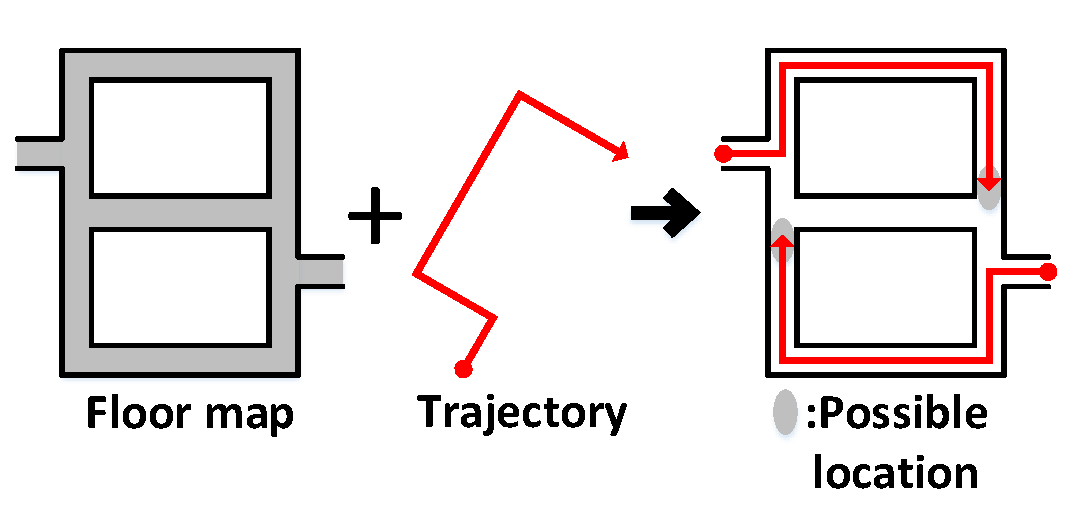
\includegraphics[width=0.9\textwidth]{apf1}\label{fig_apf_intuition1}
        \end{minipage}
        }
        \subfigure[Localization using detected landmarks.] {
        \begin{minipage}[b]{0.5\textwidth}
        \centering
        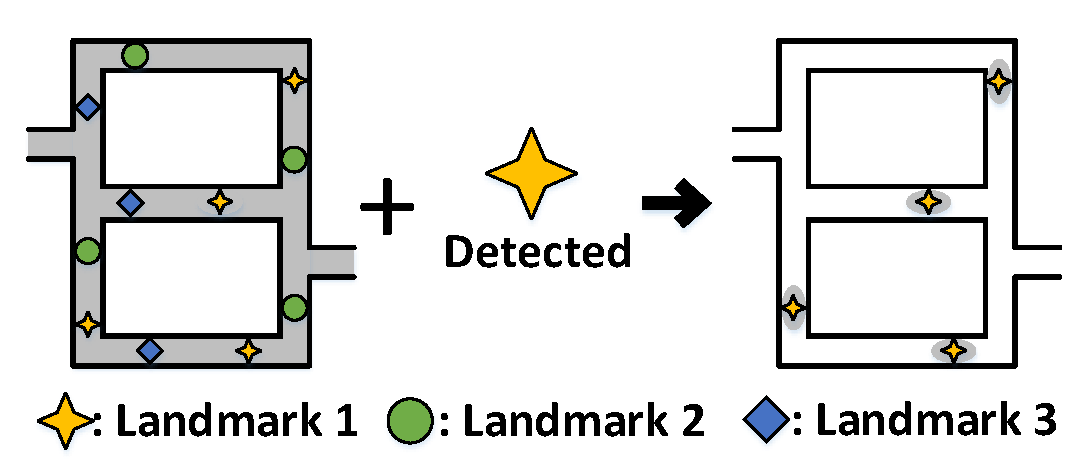
\includegraphics[width=0.9\textwidth]{apf2}\label{fig_apf_intuition2}
        \end{minipage}
        }
        \subfigure[Localization using both map constraints and detected landmarks.] {
        \begin{minipage}[b]{0.5\textwidth}
        \centering
        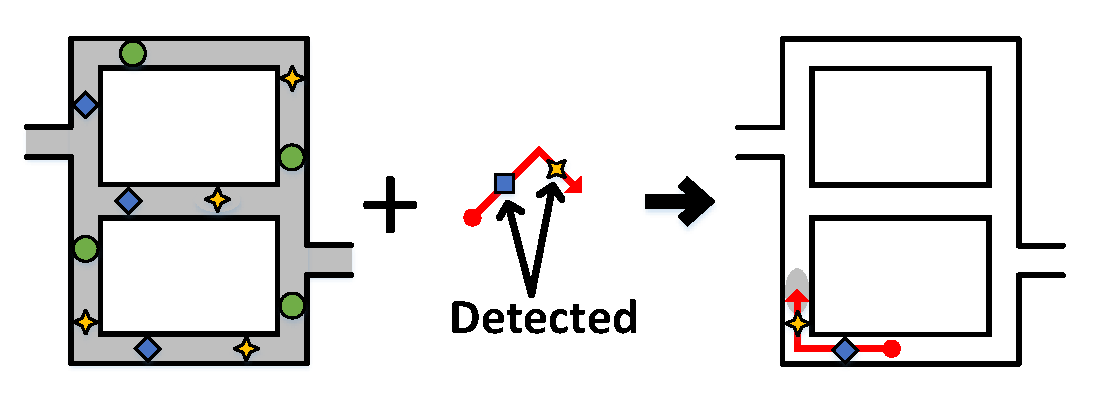
\includegraphics[width=0.9\textwidth]{apf3}\label{fig_apf_intuition3}
        \end{minipage}
        }
        \vspace{4pt}
        \caption{Intuition of localization. (a) shows that trajectories can be used for localization since only a few paths on the map could accommodate the trajectory. (b) shows that once a landmark is detected, only a few positions marked with the same kind of landmark are possible. (c) shows that using both map constraints and detected landmark could narrow down the uncertainty more quickly.}\label{fig_apf}
\end{figure}

The problem of cubically growing error in dead-reckoned trajectories \cite{Robertson:Foot-mounted_Inertial, Woodman:Pedestrian_Localisation:Foot-mounted} can also be resolved by map constraints and detected landmarks. These information provides an opportunity to re-calibrate a vehicle to correct location before the estimation error grows rapidly.

In VeLoc, we represent the uncertainty of a vehicle's states as a probability distributions over the state space. (A vehicle state includes its location, heading direction and velocity.) The tracking problem is posed as a sequential Bayesian filtering problem under the sequential importance re-sampling framework implemented by an Augmented Particle Filtering method \cite{Rai:Zee}.

We use $s_t$ to represent the state of the vehicle at time $t$, the probability distribution of vehicle states is denoted as $b(s_t)$. Bayesian filtering possesses the following two essential steps: time update and measurement update.

\textbf{Time update} is to estimate the state at time $t$ given the previous state. Different from the dead-reckoning, which simply updates the previous state with the movement, sequential Bayesian Filtering framework models the noise in movement with a probability distribution which defines the possible transitions from one state to the next as $p(s_t|s_{t-1},m_{t})$, where $m_{t}$ is the movement at time $t$.
Thus, the prior is obtained as
\begin{equation}\label{}
\overline{b}(s_t) = \int p(s_t|s_{t-1},m_{t})b(s_{t-1})ds_{t-1}.
\end{equation}

\textbf{Measurement update} is to update the probability distribution of the current state given the current measurement $m_t$. Using the Bayes rule, the posterior distribution over the state can be calculated as
\begin{equation}\label{}
b(s_t) = \eta_tp(m_t|s_t)\overline{b}(s_t),
\end{equation}
where $\eta_t$ is a normalization factor.


\subsection{Augmented Particle Filter} \label{subsec:APF_details}

Particle filter is an alternative nonparametric implementation of the sequential Bayesian filter. The key idea of the particle filter is to represent a distribution by a set of samples drawn from the distribution. The samples are called ``particles" denoted as:
\begin{equation*}
\mathcal{S}_t := \boldsymbol{s}_{t}^{(1)},...,\boldsymbol{s}_{t}^{(M)},
\end{equation*}
where M denotes the number of particles in the particle set $\mathcal{S}_t$.
Each particle $\boldsymbol{s}_t^{(i)}$($1\leq i\leq M$) is a concrete instantiation of the state at time $t$.

\textit{Augmented particles} are particles in an augmented state space. In VeLoc, the state of a particle is a five-tuple defined as $(x, y, \theta, v, d)$,
%\begin{equation*}\langle x, y, \theta, v, d\rangle\end{equation*}
where $x,y$ are position of a vehicle on a 2D floor plan, $\theta$ is the heading direction of the vehicle and $v$ is the velocity along the y-axis of the vehicle and $d$ is a binary variable, which determines the pose of the phone from two possible poses as described in Section \ref{subsec:pose_directed}.

\textbf{Time update} in our algorithm is performed by generating a hypothetical state $\boldsymbol{s}_{t}^{(m)}$ at time $t$ from its ancestor $\boldsymbol{s}_{t-1}^{(m)}$ and the current measurement $\boldsymbol{m}_t = (\omega_t, a_t)$, where $\omega$ is the rotational velocity along the z-axis of the vehicle and $a$ is the acceleration along the y-axis of the vehicle. This step involves sampling from the transition distribution $p(\boldsymbol{s}_t|\boldsymbol{s}_{t-1}, \boldsymbol{m}_t)$.
We use Gaussian distribution $\mathcal{N}(\boldsymbol{s}_t;\boldsymbol{\mu}_t, \boldsymbol{\Sigma}_t)$
to represent the transition distribution. The mean $\boldsymbol{\mu}_t$ is defined as
\begin{equation}
\boldsymbol{\mu_t} = \left(
   \begin{array}{c}
     x_{t-1} + v_{t-1}\Delta{t}\cdot\cos{\theta_{t-1}} \\
     y_{t-1} + v_{t-1}\Delta{t}\cdot\sin{\theta_{t-1}} \\
     \theta_{t-1} + \omega_t\Delta{t}\\
     v_{t-1} + a_t\Delta{t}\\
     d_{t-1} \\
   \end{array}
 \right)
\end{equation},
and $\boldsymbol{\Sigma}_t$ is diagonal matrix modeling measurement noise.

\textbf{Measurement update} in our algorithm first computes the so-called ``importance weights" (denoted as $w_{t}^{(m)}$) of each particle $\boldsymbol{s}_{t}^{(m)}$ according to $w_{t}^{(m)} \propto p(\boldsymbol{m}_t|\boldsymbol{s}_{t}^{(m)})$.
In VeLoc, the weight $w_{t}$ is computed as
\begin{equation}
w_{t} :=  \prod_{i=0}^{3}{w_{ti}},
\end{equation}
The sum of the weights at each time $t$ is normalized to one. And each $w_{ti}$ is described as follows.
\begin{itemize}
  \item \textbf{Constraints imposed by the map.} $w_{t0}$=$1$ if the position of the particle is accessible, otherwise $0$.
  \item \textbf{Detected landmarks.} For each $w_{ti}$ of the $i$-th type of landmarks ($i$=$1,2,3$), $w_{ti}$=$\mathcal{N}(D_{i}(x_t,y_t);0, \sigma_{i}^2)$ if a landmark is detected, otherwise $w_{ti}=1$. $D_{i}(x_t,y_t)$ is the distance to the closest landmark of the same type and $\sigma_{i}^2$ are parameter controlling scale of the distance.
\end{itemize}

\vspace{2mm}
The key idea of the particle filtering algorithm is \textit{sequential importance re-sampling} that draws with replacement of $M$ particles from the current set of particles according to their importance weights.
VeLoc uses Low variance sampler \cite{probabilistic} to fulfill the re-sampling task. It is worth mentioning that since re-sampling is the most time-consuming part of the algorithm, VeLoc does not perform re-sampling after every time step, instead, it maintains the importance weight for each particle, and the weights updated multiplicatively until the next re-sampling. In Veloc, re-sampling is performed every 10 time steps.


\subsection{Vehicle State Estimation} \label{subsec:APF_effect}
Using augmented particle filter as described above, VeLoc can estimate the state of the vehicle, including its location.
To illustrate how VeLoc works, we use an example scenario to drive the process of realtime tracking. Figure \ref{fig_route} shows the map of an underground parking lot with an actual route denoted by 7 key points (i.e., A to G as shown with time stamps).

\begin{figure}[htbp]
\centering
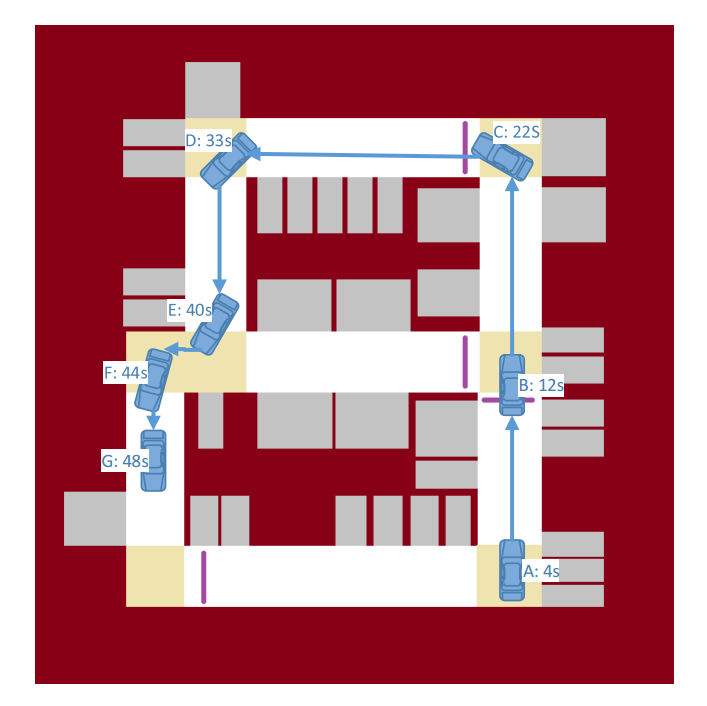
\includegraphics[scale=.3]{route.png}
\caption{Map of the example scenario shown with an actual route denoted by 7 key points and the times when the vehicle passes them. The vehicle starts at A and stops at G. }\label{fig_route}
\end{figure}

\textbf{Experiment with the initial position and heading direction of the vehicle.}
We first show in Figure \ref{fig_case1} the positions of all the particles as time goes by. Since the initial position and heading direction are known, Figure \ref{fig_case1}(a) shows that all the particles are initialized around the entrance. Figure \ref{fig_case1}(b) and (c) show that the particles diverge due to growing uncertainties caused by noises in measurements. Figure \ref{fig_case1}(d) shows that particles slightly come closer after a speed bump detection reduces the uncertainty. After a left turn, the uncertainty is greatly reduced and particles come very close (Figure \ref{fig_case1}(e)-(g)). In Figure \ref{fig_case1}(f), particles with too great or too slow speeds will hit either the front wall or side wall, and eventually disappear. Only those with appropriate speed around that of the ground truth will be able to make the left turn and continue traveling along the top isle. Figure \ref{fig_case1}(h)-(k) show how three more turns each cause more concentration of the particles. Figure \ref{fig_case1}(l) shows the final position of all the particles and the average position is shown with a red point. Compared to the actual route (Figure \ref{fig_route}), VeLocE produces a quite accurate final location.

%\begin{figure}[htbp]
\begin{figure}[t]
%\begin{tabular}{cc}
\centering
\begin{minipage}{0.32\linewidth}
  \centerline{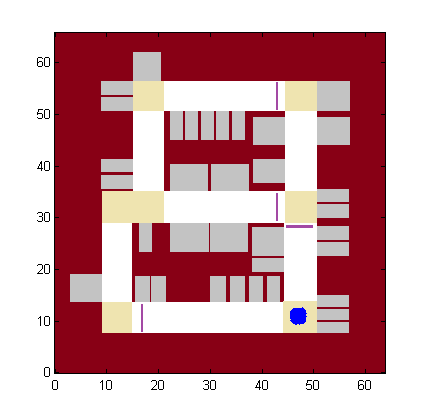
\includegraphics[scale=.3]{fig1-1.png}}
  \centerline{(a)}
\end{minipage}
\begin{minipage}{0.32\linewidth}
  \centerline{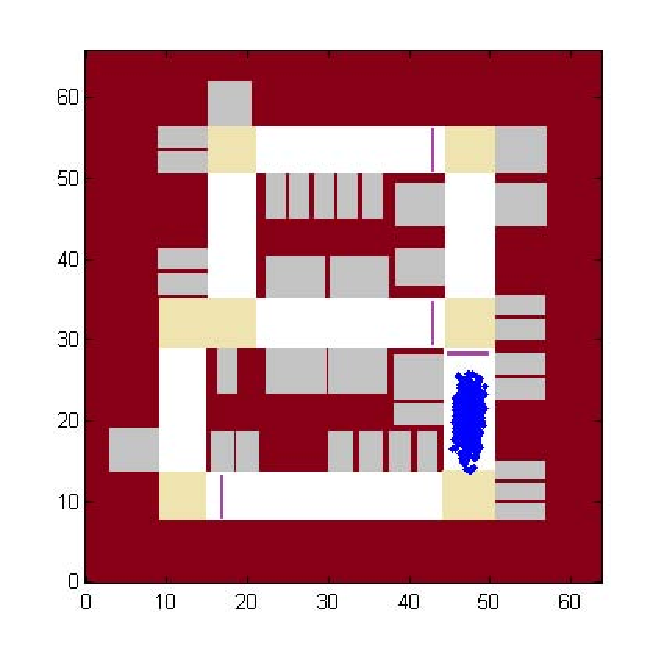
\includegraphics[scale=.3]{fig1-2.pdf}}
  \centerline{(b)}
\end{minipage}
\begin{minipage}{0.32\linewidth}
  \centerline{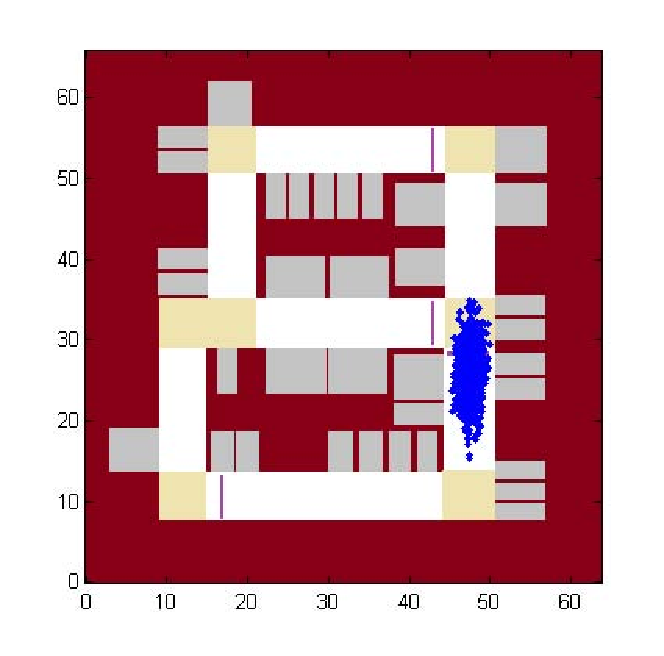
\includegraphics[scale=.3]{fig1-3.pdf}}
  \centerline{(c)}
\end{minipage}
\centering
\begin{minipage}{0.32\linewidth}
  \centerline{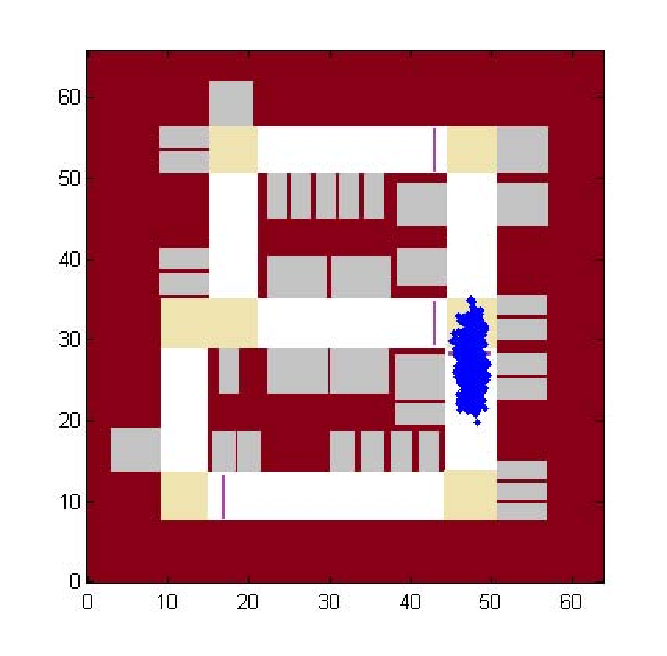
\includegraphics[scale=.3]{fig1-4.pdf}}
  \centerline{(d)}
\end{minipage}
\begin{minipage}{0.32\linewidth}
  \centerline{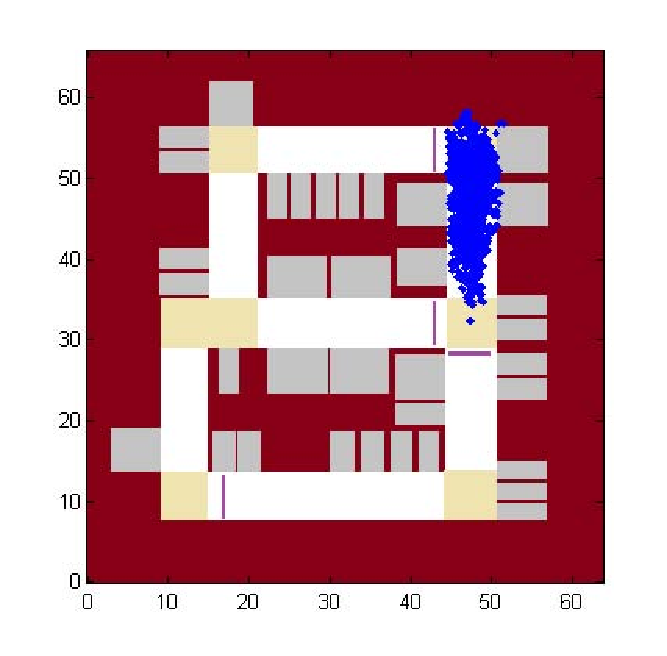
\includegraphics[scale=.3]{fig1-5.pdf}}
  \centerline{(e)}
\end{minipage}
\begin{minipage}{0.32\linewidth}
  \centerline{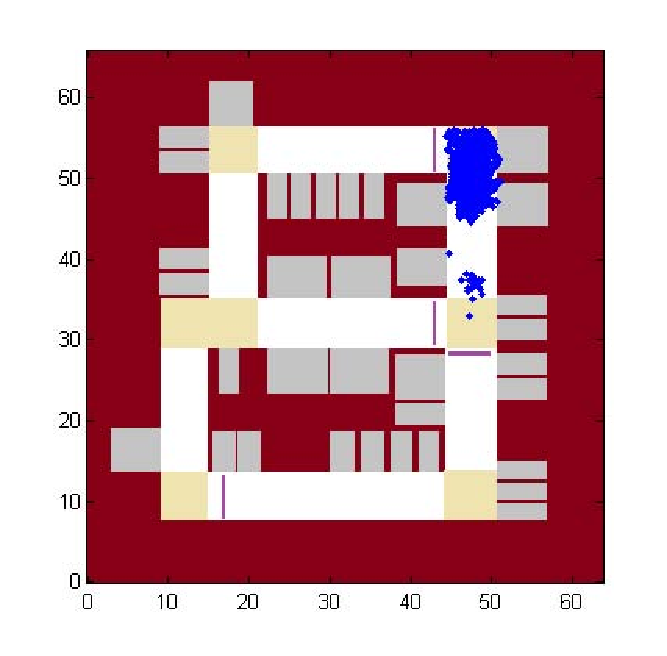
\includegraphics[scale=.3]{fig1-6.pdf}}
  \centerline{(f)}
\end{minipage}
\centering
\begin{minipage}{0.32\linewidth}
  \centerline{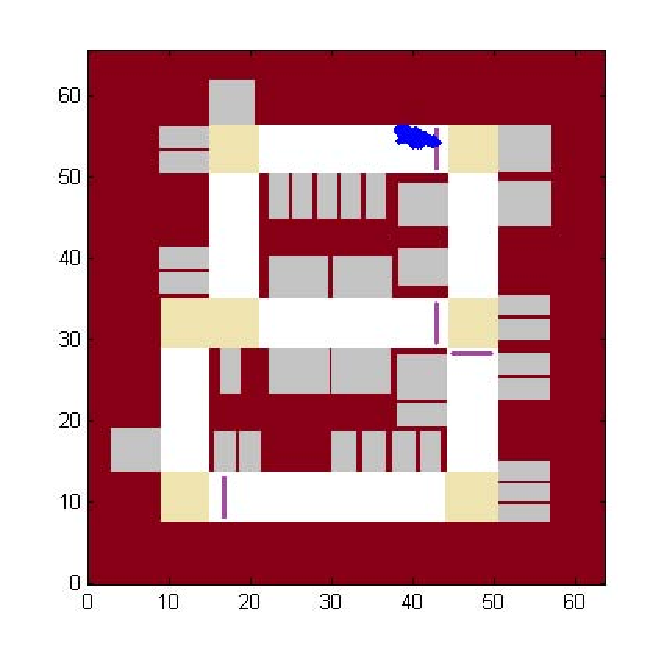
\includegraphics[scale=.3]{fig1-7.pdf}}
  \centerline{(g)}
\end{minipage}
\begin{minipage}{0.32\linewidth}
  \centerline{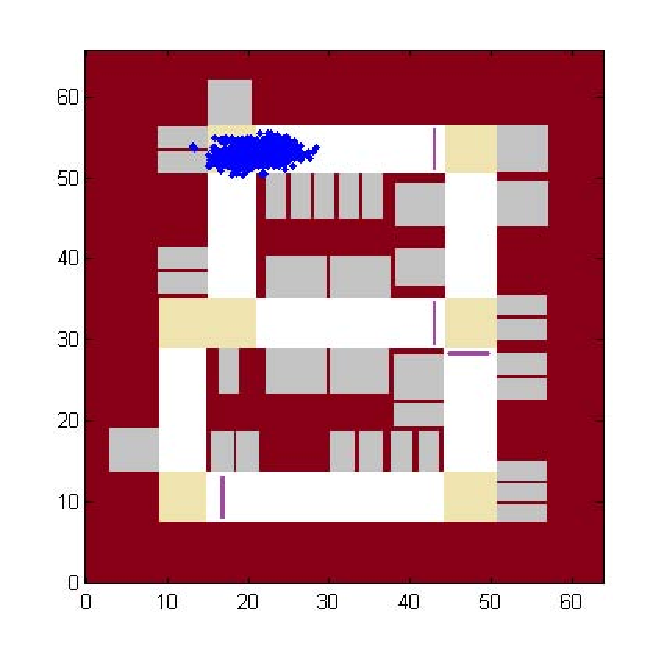
\includegraphics[scale=.3]{fig1-8.pdf}}
  \centerline{(h)}
\end{minipage}
\begin{minipage}{0.32\linewidth}
  \centerline{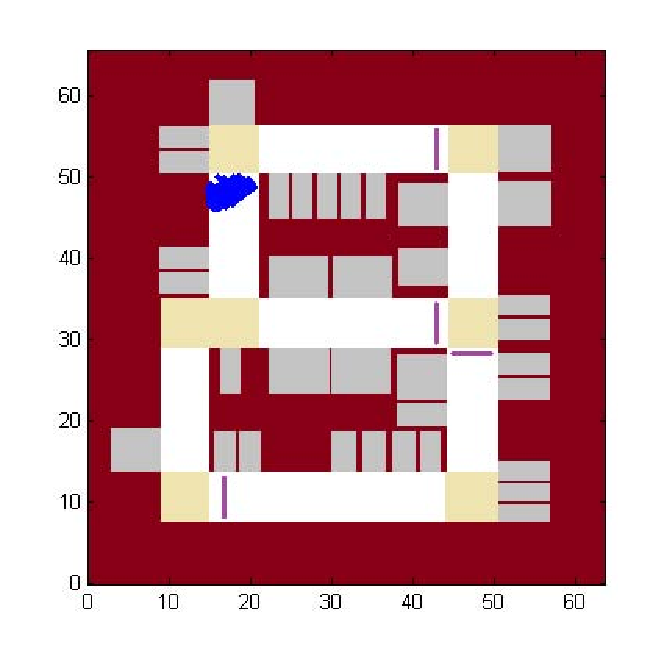
\includegraphics[scale=.3]{fig1-9.pdf}}
  \centerline{(i)}
\end{minipage}
\centering
\begin{minipage}{0.32\linewidth}
  \centerline{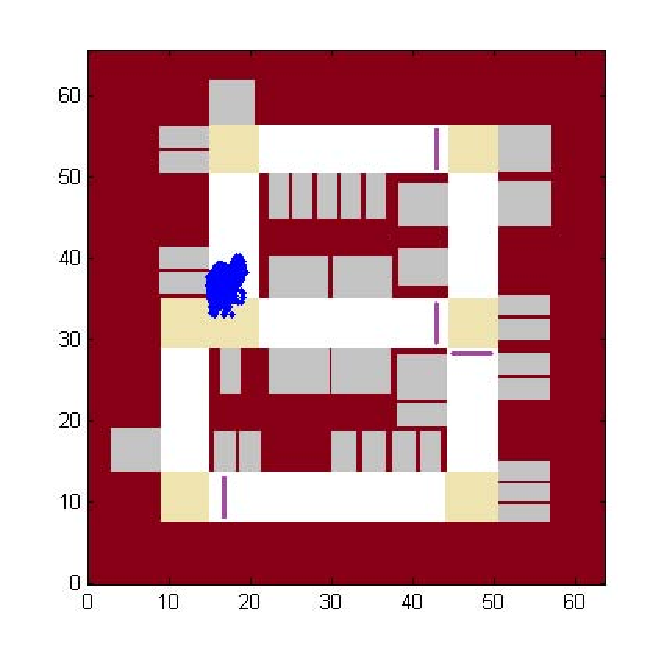
\includegraphics[scale=.3]{fig1-10.pdf}}
  \centerline{(j)}
\end{minipage}
\begin{minipage}{0.32\linewidth}
  \centerline{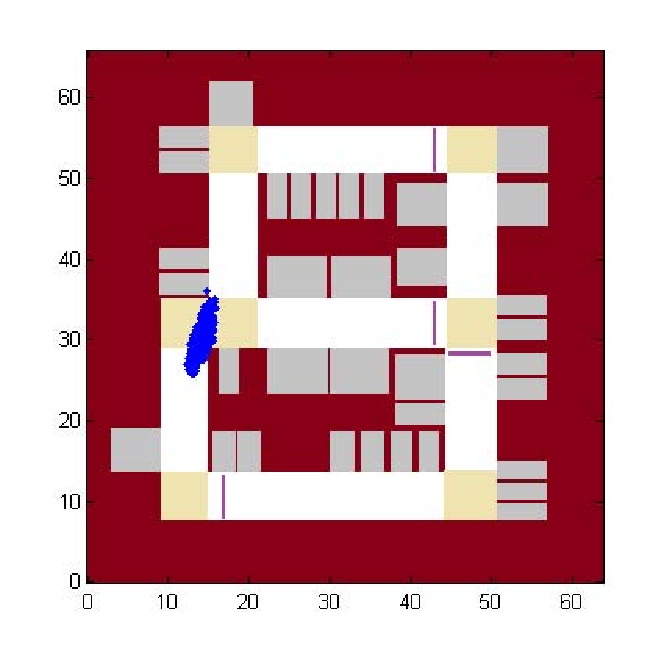
\includegraphics[scale=.3]{fig1-11.pdf}}
  \centerline{(k)}
\end{minipage}
\begin{minipage}{0.32\linewidth}
  \centerline{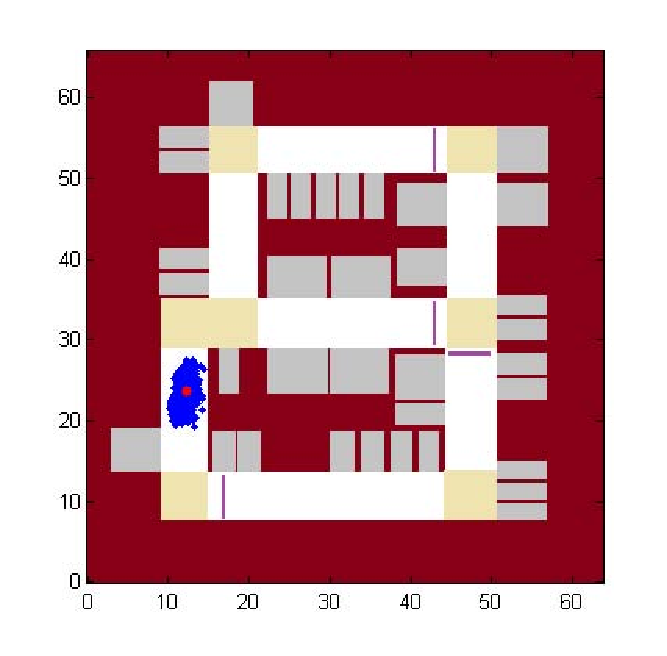
\includegraphics[scale=.3]{fig1-12.pdf}}
  \centerline{(l)}
\end{minipage}
%\end{tabular}
\vspace{5pt}
\caption{Particles over time with initial position and heading direction of the vehicle.}\label{fig_case1}
\end{figure}

\textbf{Experiment with only the initial heading direction of the vehicle.}
Figure \ref{fig_case2} shows the process if the initial position is unknown but the initial heading direction is somehow known (e.g, using compass to find which of the four directions imposed by the parking lot aisles is the most likely one). As shown in Figure \ref{fig_case2}(a), particles are initialized everywhere in the parking lot. As the vehicle starts moving up, constraints imposed by the map filter out many particles that would hit walls when moving up (shown in Figure \ref{fig_case2}(b)). Figure \ref{fig_case2}(c) shows more particles are eliminated when a landmark (i.e., speed bump) is detected, and only those just passing around a speed bump can survive. Figure \ref{fig_case2}(d)(e) show that the detected left turn eliminate many particles and the remaining ones cluster around the corner. Figure \ref{fig_case2}(e) looks similar to Figure \ref{fig_case1}(g), showing that VeLoc succeeds in estimating the state of the vehicle without the initial position. From there the process is similar to the previous one. Figure \ref{fig_case2}(f) shows the final position of all the particles and the average position is shown with a red point, which is very accurate as well. We can also trace back to determine the initial position of the vehicle which is not known at the beginning. % Comparing with the route shown in Figure \ref{fig_route} ), VeLocE gets a very accurate result in localization problem without initial position.


\begin{figure}[htbp]
%\begin{tabular}{cc}
\begin{minipage}{0.32\linewidth}
\centering
  \centerline{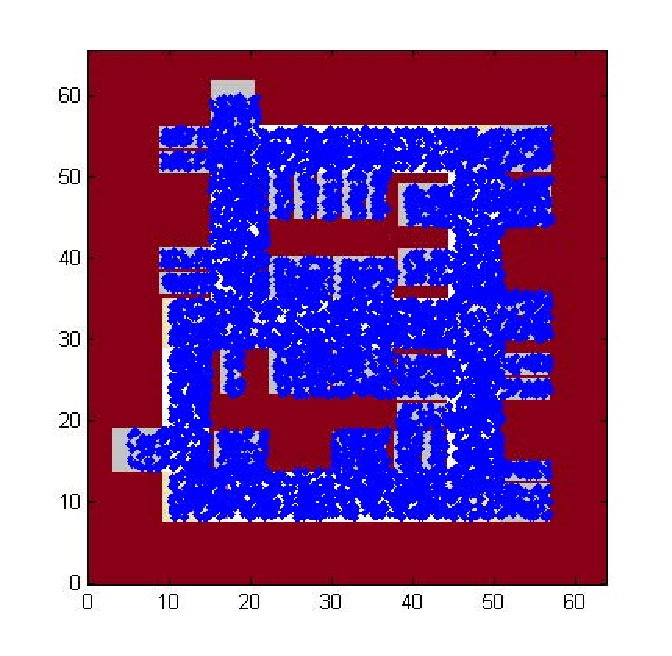
\includegraphics[scale=.3]{fig2-1.pdf}}
  \centerline{(a)}
\end{minipage}
\begin{minipage}{0.32\linewidth}
  \centerline{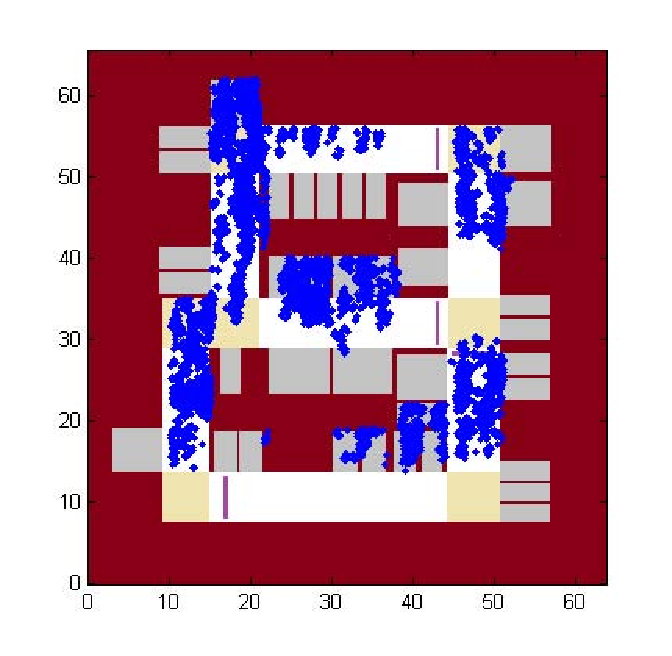
\includegraphics[scale=.3]{fig2-2.pdf}}
  \centerline{(b)}
\end{minipage}
\begin{minipage}{0.32\linewidth}
  \centerline{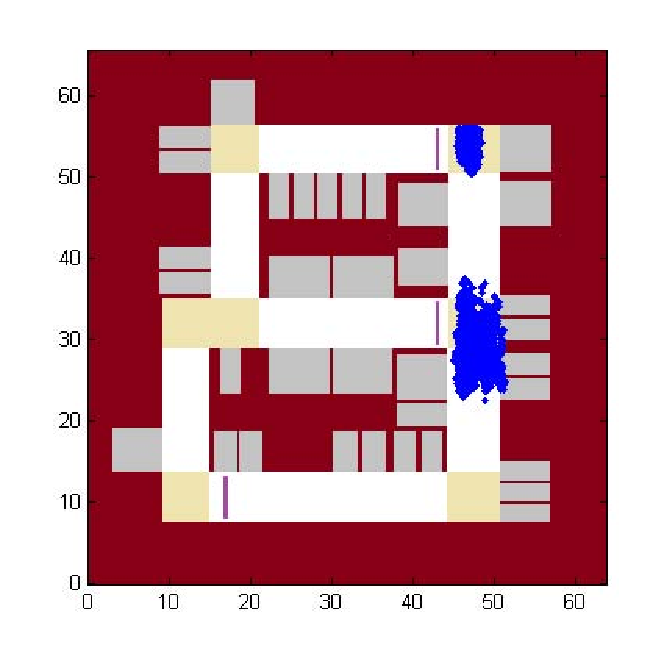
\includegraphics[scale=.3]{fig2-3.pdf}}
  \centerline{(c)}
\end{minipage}
\centering
\begin{minipage}{0.32\linewidth}
  \centerline{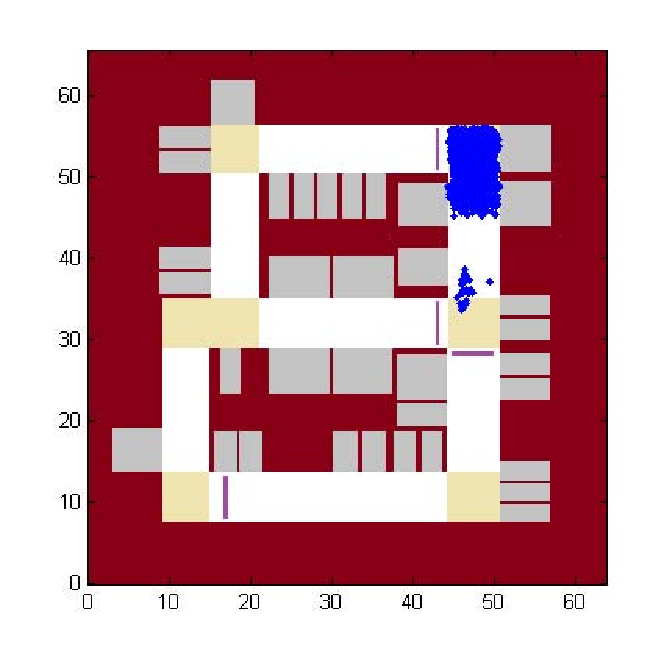
\includegraphics[scale=.3]{fig2-4.pdf}}
  \centerline{(d)}
\end{minipage}
\begin{minipage}{0.32\linewidth}
  \centerline{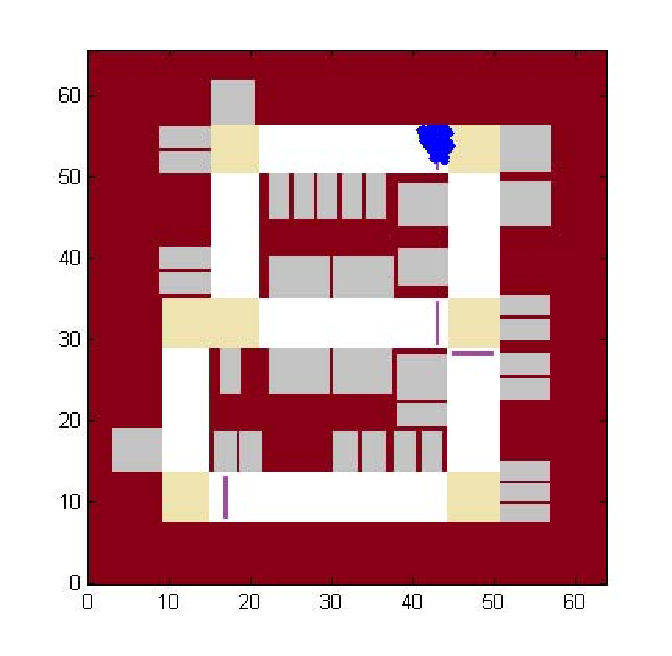
\includegraphics[scale=.3]{fig2-5.pdf}}
  \centerline{(e)}
\end{minipage}
\begin{minipage}{0.32\linewidth}
  \centerline{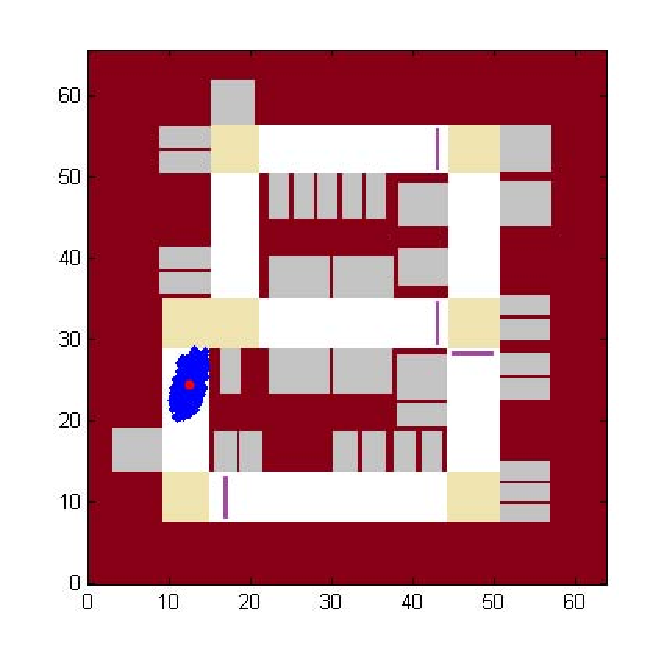
\includegraphics[scale=.3]{fig2-6.pdf}}
  \centerline{(f)}
\end{minipage}
%\end{tabular}
\vspace{5pt}
\caption{Particles over time with only the initial heading of the vehicle.}\label{fig_case2}
\end{figure}

\textbf{Experiment with neither the initial position nor heading direction of the vehicle.}
Figure \ref{fig_case3} shows the results if neither the initial position nor the heading direction is unknown. VeLocE is still able to estimate the true state of the vehicle but it may take a litter longer to converge. As shown in Figure \ref{fig_case3}(a), particles are initialized everywhere in the parking lot. Constraints imposed by the map (i.e., walls) filter out some particles but compared to Figure \ref{fig_case2}(b) they are still widely distributed (shown in Figure \ref{fig_case3}(b)). This is because the lack of heading direction gives more particles the chance to survive. Figure \ref{fig_case3}(c) shows how particles converge quickly when a landmark of speed bump eliminate those without a bump nearby. However, compared to Figure \ref{fig_case2}(c), they are still distributed more widely. In Figure \ref{fig_case3}(d), particles traveling in horizontal directions are eliminated because the vehicle keeps moving upwards, but those traveling vertically become more dispersed. Figure \ref{fig_case3}(e) shows that how a left turn detected remove most of the particles and leaving only close to the true location, the upper right corner. Figure \ref{fig_case3}(f) again shows the final positions of all the particles and their average position shown with a red point. From this example, we can see that VeLocE can produce very accurate results even both the initial position and the heading direction are unknown.

\begin{figure}[htbp]
%\begin{tabular}{cc}
\begin{minipage}{0.32\linewidth}
\centering
  \centerline{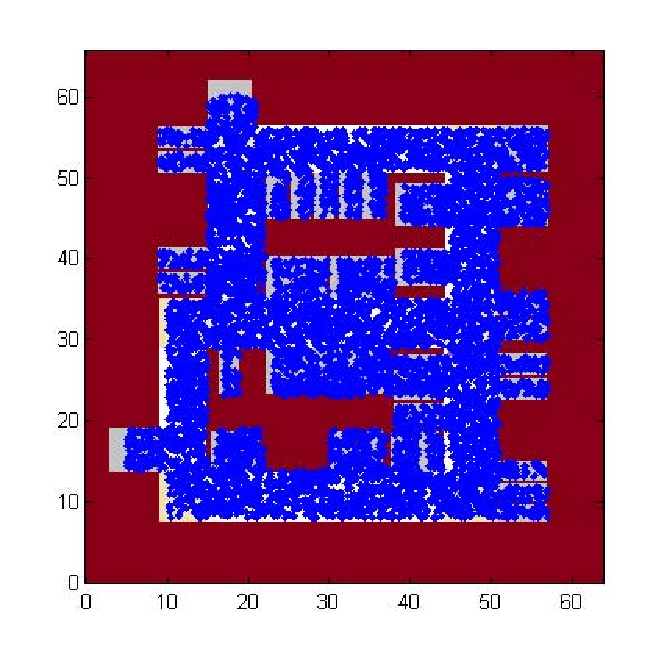
\includegraphics[scale=.3]{fig3-1.pdf}}
  \centerline{(a)}
\end{minipage}
\begin{minipage}{0.32\linewidth}
  \centerline{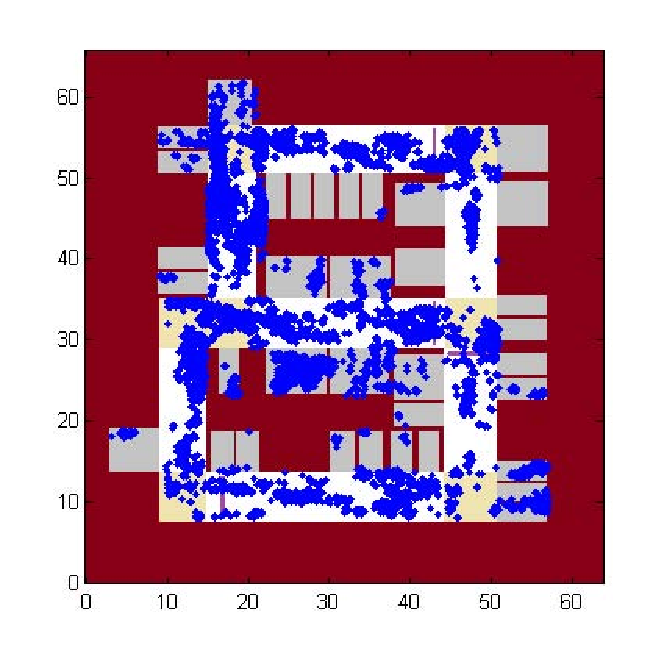
\includegraphics[scale=.3]{fig3-2.pdf}}
  \centerline{(b)}
\end{minipage}
\begin{minipage}{0.32\linewidth}
  \centerline{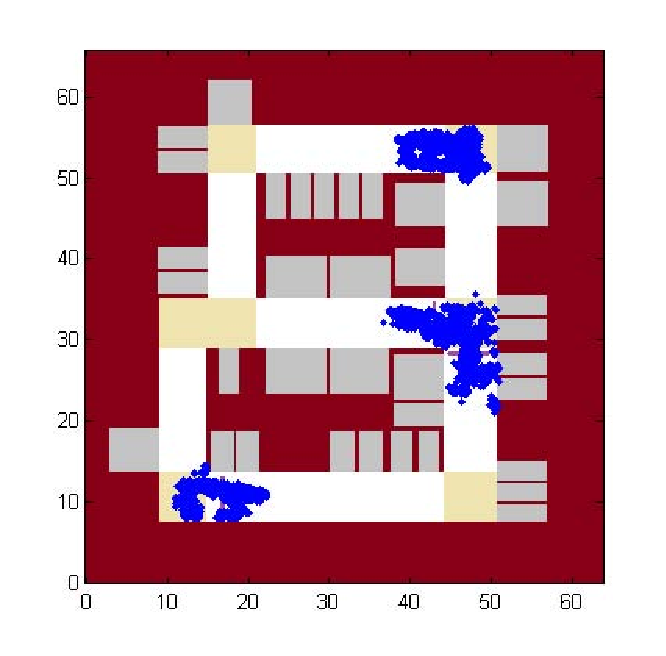
\includegraphics[scale=.3]{fig3-3.pdf}}
  \centerline{(c)}
\end{minipage}
\centering
\begin{minipage}{0.32\linewidth}
  \centerline{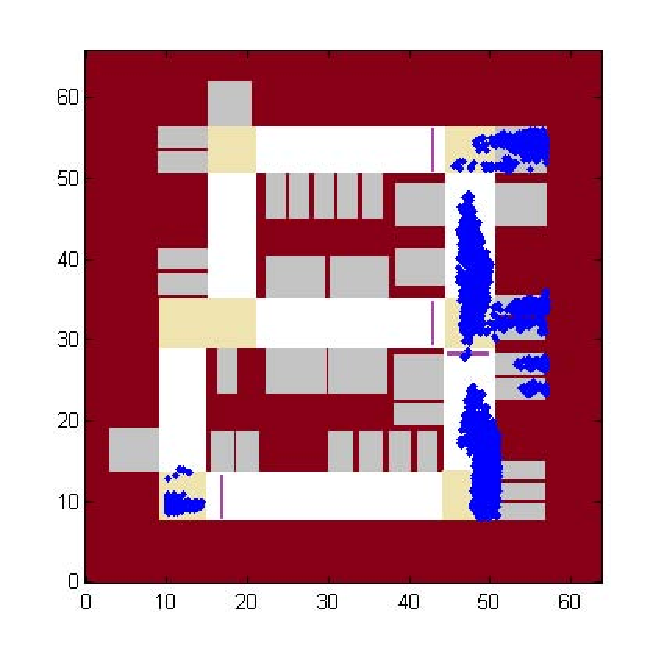
\includegraphics[scale=.3]{fig3-4.pdf}}
  \centerline{(d)}
\end{minipage}
\begin{minipage}{0.32\linewidth}
  \centerline{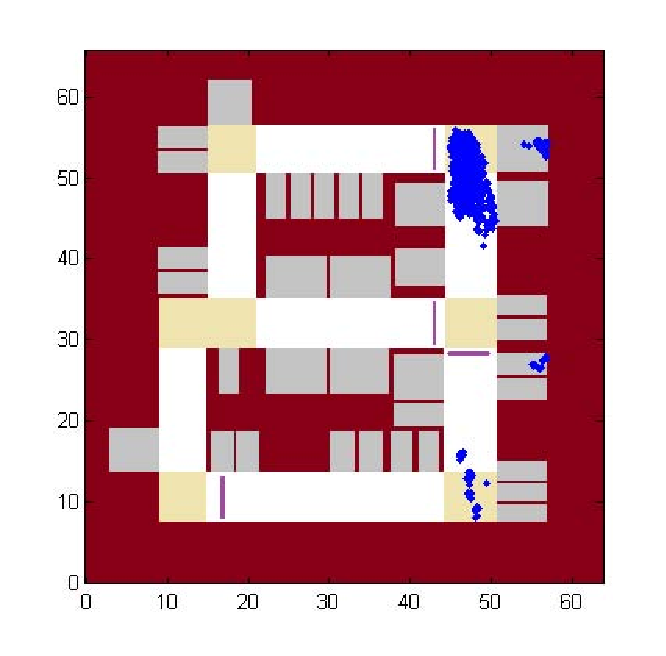
\includegraphics[scale=.3]{fig3-5.pdf}}
  \centerline{(e)}
\end{minipage}
\begin{minipage}{0.32\linewidth}
  \centerline{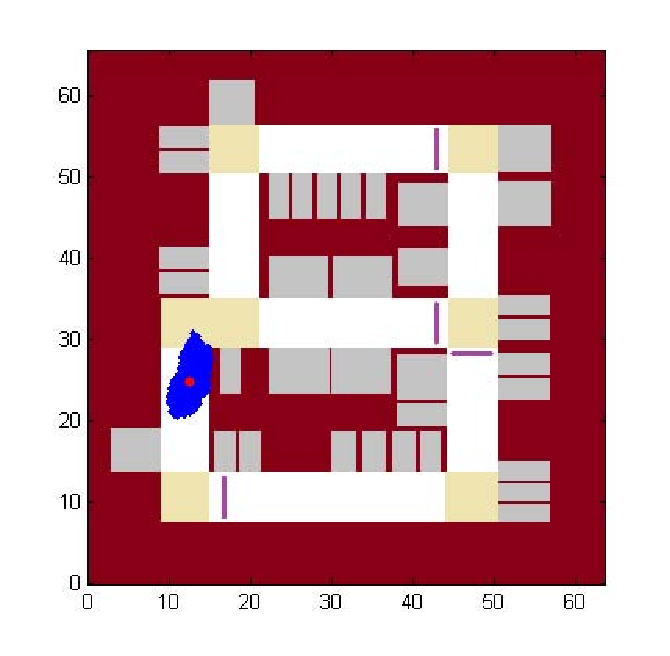
\includegraphics[scale=.3]{fig3-6.pdf}}
  \centerline{(f)}
\end{minipage}
%\end{tabular}
\vspace{5pt}
\caption{Particles over time with neither the initial position or initial heading direction of the vehicle.}\label{fig_case3}
\end{figure}




































\iffalse
In this section we describe how VeLocE uses Augmented Particle Filter (APF) to track the vehicles�� paths as they move in a parking lot. We will first introduce the APF algorithm and then describe the time update and the measurement update, which are the two essential steps in all Bayes Filter based algorithms.\\

Particle filter is an alternative nonparametric implementation of the Bayes filter. The key idea of the particle filter is to represent a distribution by a set of samples drawn from this distribution. In particle filters, the samples of a posterior distribution are called \textit{particles} and are denoted as:
\begin{equation*}\mathcal{X}_t := \boldsymbol{x}_{t}^{[1]},\boldsymbol{x}_{t}^{[2]},...,\boldsymbol{x}_{t}^{[M]}\end{equation*}

Each particle $\boldsymbol{x}_t^{[m]}$(with $1\leq m\leq M$)s a concrete instantiation of the state at time t, that is, a hypothesis as to what the true world state may be at time t. Here M denotes the number of particles in the particle set $\mathcal{X}_t$.\\

\textit{Augmented particles} are novel particles that also incorporate the uncertainty in other aspects such as the direction of the smartphone and the velocity of the vehicle.\\

Just like all other Bayes filter algorithms, APF algorithm constructs the distribution at time t recursively from the distribution one time step earlier. Since beliefs are represented by sets of particles, this means that APF construct the particle set $\mathcal{X}_t$ recursively from the set $\mathcal{X}_{t-1}$.\\

The following is the pseudocode for APF algorithm in VeLocE while $\boldsymbol{u}_t$ and $\boldsymbol{z}_t$ are control and measurement at time t.
\begin{algorithm}[htb]
\caption{$ Augmented\underline{\;}Particle\underline{\;}Filter(\mathcal{X}_{t-1}, \boldsymbol{u}_t, \boldsymbol{z}_t) $}
\begin{algorithmic}[1]
\STATE $\overline{\mathcal{X}}_t = \mathcal{X}_t = \emptyset$
\FOR{$m=1$ to $M$}
\STATE sample $\boldsymbol{x}_{t}^{[m]}\thicksim p(\boldsymbol{x}_t|\boldsymbol{u}_t, \boldsymbol{x}_{t-1}^{[m]})$
\STATE $\overline{\mathcal{X}}_t = \overline{\mathcal{X}}_t \cup \{\boldsymbol{x}_{t}^{[m]}\}$
\ENDFOR
\FOR{$m=1$ to $M$}
\STATE $w_{t}^{[m]} = p(\boldsymbol{z}_t|\boldsymbol{x}_{t}^{[m]})$
\ENDFOR
\FOR{$m=1$ to $M$}
\STATE draw $\boldsymbol{x}_{t}^{[i]}$ from $\overline{\mathcal{X}}_t$ with probability $\varpropto w_{t}^{[i]}$
\STATE $\mathcal{X}_t = \mathcal{X}_t \cup \{\boldsymbol{x}_{t}^{[i]}\}$
\ENDFOR
\RETURN $\mathcal{X}_t$
\end{algorithmic}
\end{algorithm}

\textit{Time update}, which is also known as \textit{control update}, is shown in Lines 2 through 5 while \textit{measurement update} is shown in Lines 6 through 12.\\

During the time update, APF generates a hypothetical state $\boldsymbol{x}_{t}^{[m]}$ for time t based on the particle $\boldsymbol{x}_{t-1}^{[m]}$ and the control $\boldsymbol{u}_t$. The resulting sample is indexed by $m$, indicating that it is generated from the $m$-th particle in $\mathcal{X}_{t-1}$. This step involves sampling from the transition distribution $p(\boldsymbol{x}_t|\boldsymbol{u}_t, \boldsymbol{x}_{t-1}^{[m]})$ which is not always possible for arbitrary distributions.\\

During the measurement update, APF first calculates for each particle $\boldsymbol{x}_{t}^{[m]}$ the so-called importance weights, denoted $w_{t}^{[m]}$. Importance weights are used to incorporate the measurement $\boldsymbol{z}_t$ into the particle set. The importance weight, thus, is the probability of the measurement $\boldsymbol{z}_t$ under the particle $\boldsymbol{x}_{t}^{[m]}$, that is, $w_{t}^{[m]} \propto p(\boldsymbol{z}_t|\boldsymbol{x}_{t}^{[m]})$. The real ``trick'' of the particle filter algorithm occurs in Lines 9 through 12 which implements what is known as \textit{resampling} or \textit{importance resampling}. The algorithm draws with replacement $M$ particles from the temporary Set $\overline{\mathcal{X}}_t$ . The probability of drawing each particle is given by its importance weight. By incorporating the importance weights into the resampling process, the distribution of the particles changes over time.\\

In the rest of this section, we describe the transition distribution, importance weights and resampling method in VeLocE.

\subsubsection{Transition Distribution}
To define the transition distribution in VeLocE, we need first introduce the state of a particle and the control. The state of a particle is a four-dimension vector defined as follows:
\begin{equation*}\langle x, y, \theta, v\rangle\end{equation*}
where $x,y$ are position of the vehicle, $\theta$ is the heading direction of the vehicle and $v$ is the velocity along the y-axis of the vehicle shown in Figure \ref{fig_state}. The control is defined as follows:
\begin{equation*}\langle w, a\rangle\end{equation*}
where $w$ is the rotational velocity along the z-axis of the vehicle and $a$ is the acceleration along the y-axis of the vehicle shown in Figure \ref{fig_state}.

\begin{figure}[htbp]
\centering
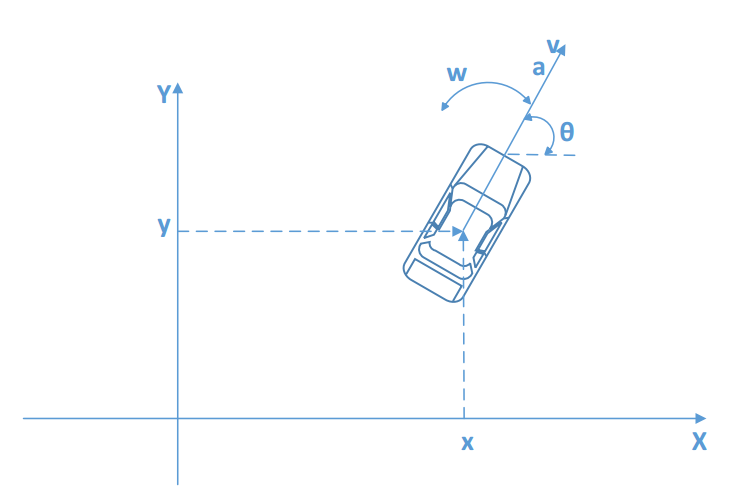
\includegraphics[scale=.46]{state.png}
\caption{State and Control}\label{fig_state}
\end{figure}

We use four-dimension Gaussian distribution
\begin{equation} \mathcal{N}(\boldsymbol{x}_t|\boldsymbol{\mu}_t, \boldsymbol{\Sigma}_t) = \frac{1}{4\pi^2}\frac{1}{|\boldsymbol{\Sigma}_t|^\frac{1}{2}} e^{-\frac{1}{2}(\boldsymbol{x}_t-\boldsymbol{\mu}_t)^{T}\boldsymbol{\Sigma}_t^{-1}(\boldsymbol{x}_t-\boldsymbol{\mu}_t)}\end{equation}
to represent the transition distribution in VeLocE.\\

$\boldsymbol{\mu}_t$ is defined as follows:
\begin{equation}\boldsymbol{\mu_t} = \boldsymbol{G}(\boldsymbol{x}_{t-1}) + \boldsymbol{H}(\boldsymbol{z}_{t})\end{equation}
where
\begin{equation}
\boldsymbol{G}(\boldsymbol{x}_{t-1}) = \boldsymbol{G}(\left(
                                                        \begin{array}{c}
                                                          x_{t-1} \\
                                                          y_{t-1} \\
                                                          \theta_{t-1} \\
                                                          v_{t-1} \\
                                                        \end{array}
                                                      \right))
=\left(
   \begin{array}{c}
     x_{t-1} + v_{t-1}\Delta{t}\cdot\cos{\theta_{t-1}} \\
     y_{t-1} + v_{t-1}\Delta{t}\cdot\sin{\theta_{t-1}} \\
     \theta_{t-1} \\
     v_{t-1} \\
   \end{array}
 \right)
\end{equation}
and
\begin{equation}
\boldsymbol{H}(\boldsymbol{z}_{t}) = \boldsymbol{H}(\left(
                                                      \begin{array}{c}
                                                        w_t \\
                                                        a_t \\
                                                      \end{array}
                                                    \right))
=\left(
   \begin{array}{c}
     0\\
     0\\
     w_t\Delta{t} \\
     a_t\Delta{t} \\
   \end{array}
 \right)
\end{equation}

$\boldsymbol{\Sigma}_t$ is defined as follows:
\begin{equation}
\boldsymbol{\Sigma}_t = \left(
                          \begin{array}{cccc}
                            \sigma_x^2 & 0 & 0 & 0 \\
                            0 & \sigma_y^2 & 0 & 0 \\
                            0 & 0 & \sigma_{\theta}^2 & 0 \\
                            0 & 0 & 0 & \sigma_v^2 \\
                          \end{array}
                        \right)
\end{equation}
where all $\sigma^2$ describe measurement noise.

\subsubsection{Importance Weights}
We define the measurement $\boldsymbol{z}_t$ in VeLocE as follows:
\begin{equation*}\langle road\;anomaly, turning, slope, moving, reachability \rangle\end{equation*}
Every element can take 0 or 1 so that $\boldsymbol{z}_t\in[0,1]^5$. The first three elements are outputs of PD indicating whether a landmark is encountered. The element $moving$ is also one output of PD indicating whether the vehicle is moving. The last element $reachability$ indicates whether the vehicle can reach the current position and obviously is it always 1.\\

To calculate the probability $p(\boldsymbol{z}_t|\boldsymbol{x}_{t}^{[m]})$, we assume that elements of $\boldsymbol{z}_t$ are independent so that:
\begin{equation}
p(\boldsymbol{z}_t|\boldsymbol{x}_{t}^{[m]}) = \prod_{i=1}^{5}{p(z_{ti}|\boldsymbol{x}_{t}^{[m]})}
\end{equation}

As described before, $w_{t}^{[m]} \propto p(\boldsymbol{z}_t|\boldsymbol{x}_{t}^{[m]})$. We can also calculate $w_{t}^{[m]}$ as:
\begin{equation}
w_{t}^{[m]} :=  \prod_{i=1}^{5}{w_{ti}^{[m]}}
\end{equation}
where for $1\leq{i}\leq5$
\begin{equation}
w_{ti}^{[m]} \propto p(z_{ti}|\boldsymbol{x}_{t}^{[m]})
\end{equation}\\

In the rest of this part we will introduce the way to calculate $w_{ti}^{[m]}$ for $1\leq{i}\leq5$.\\

$w_{t1}^{[m]}$ for $road\;anomaly$: Since all the road anomalies are noted on the map, we can calculate for every position $(x,y)$ the closest distance to any road anomalies $dist_{RA}(x,y)$. $w_{t1}^{[m]}$ is defined as follows:

\begin{equation}
w_{t1}^{[m]} = \left\{
                   \begin{array}{ll}
                     1, & \hbox{$road\;anomaly = 0$;} \\
                     \mathcal{N}(dist_{RA}(x_{t1}^{[m]},x_{t2}^{[m]})|0, \sigma_{RA}^2), & \hbox{$road\;anomaly = 1$.}
                   \end{array}
                 \right.
\end{equation}
When a road anomaly is detected, a particle which is closer to a road anomaly noted on the map will have a bigger importance weight.\\

Similarly, $w_{t2}^{[m]}$ and $w_{t2}^{[m]}$ can be defined as follows:
\begin{equation}
w_{t2}^{[m]} = \left\{
                   \begin{array}{ll}
                     1, & \hbox{$turning = 0$;} \\
                     \mathcal{N}(dist_{TU}(x_{t1}^{[m]},x_{t2}^{[m]})|0, \sigma_{TU}^2), & \hbox{$turning = 1$.}
                   \end{array}
                 \right.
\end{equation}

\begin{equation}
w_{t3}^{[m]} = \left\{
                   \begin{array}{ll}
                     1, & \hbox{$slope = 0$;} \\
                     \mathcal{N}(dist_{SL}(x_{t1}^{[m]},x_{t2}^{[m]})|0, \sigma_{SL}^2), & \hbox{$slope = 1$.}
                   \end{array}
                 \right.
\end{equation}

$w_{t4}^{[m]}$ for $moving$: When the vehicle is detected to be immobile, a particle with velocity close to 0 should have a big importance weight. Thus, we define $w_{t4}^{[m]}$ as follows:
\begin{equation}
w_{t4}^{[m]} = \left\{
                   \begin{array}{ll}
                     \mathcal{N}(x_{t4}^{[m]}|0, \sigma_{MV}^2), & \hbox{$moving = 0$;} \\
                     1, & \hbox{$moving = 1$.}
                   \end{array}
                 \right.
\end{equation} \\

$w_{t5}^{[m]}$ for $reachability$: To use the constraints imposed by the map, we give a 0 importance weight to those particles whose positions are noted not able to reach on the map. Assume that $reach(x,y)$ is the information provided by the map to indicate whether the position $(x,y)$ is able to reach. Thus, we define $w_{t5}^{[m]}$ as follows:

\begin{equation}
w_{t5}^{[m]} =
\begin{cases}
1, \hbox{ reach($x_{t1}^{[m]}, x_{t2}^{[m]})=0, reachability=0$;}\\
0, \hbox{ reach($x_{t1}^{[m]}, x_{t2}^{[m]})=0, reachability=1$;}\\
0, \hbox{ reach($x_{t1}^{[m]}, x_{t2}^{[m]})=1, reachability=0$;}\\
1, \hbox{ reach($x_{t1}^{[m]}, x_{t2}^{[m]})=1, reachability=1$;}
\end{cases}
\end{equation}

\subsubsection{Resampling Method}
VeLocE uses Low variance sampler\cite{probabilistic} to fulfill the resampling task. It is worth mentioning that since resampling is most time-consuming part of the algorithm, VeLocE does not perform resampling after every update. VeLocE maintains for each particle an importance weight that is initialized by 1 after resampling and updated multiplicatively untill next resampling. In VelocE, resampling is performed every 10 updates.


\begin{figure*}[htbp]
%\begin{tabular}{cc}
\begin{minipage}{0.32\linewidth}
  \centerline{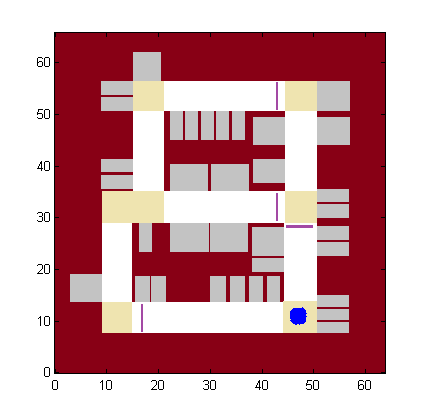
\includegraphics[scale=.3]{fig1-1.png}}
  \centerline{(a)}
\end{minipage}
\begin{minipage}{0.32\linewidth}
  \centerline{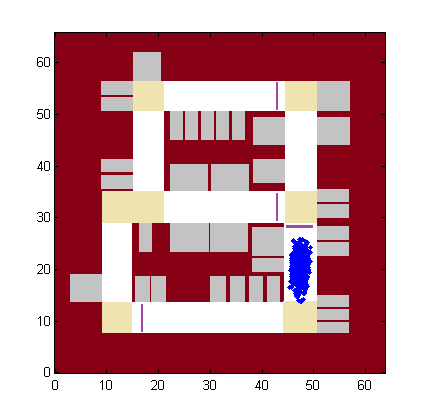
\includegraphics[scale=.3]{fig1-2.png}}
  \centerline{(b)}
\end{minipage}
\begin{minipage}{0.32\linewidth}
  \centerline{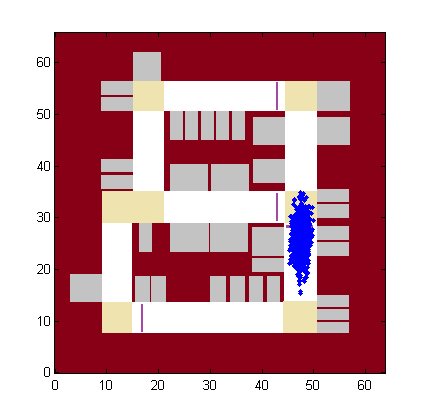
\includegraphics[scale=.3]{fig1-3.png}}
  \centerline{(c)}
\end{minipage}
\begin{minipage}{0.32\linewidth}
  \centerline{\includegraphics[scale=.3]{fig1-4.png}}
  \centerline{(d)}
\end{minipage}
\begin{minipage}{0.32\linewidth}
  \centerline{\includegraphics[scale=.3]{fig1-5.png}}
  \centerline{(e)}
\end{minipage}
\begin{minipage}{0.32\linewidth}
  \centerline{\includegraphics[scale=.3]{fig1-6.png}}
  \centerline{(f)}
\end{minipage}
\begin{minipage}{0.32\linewidth}
  \centerline{\includegraphics[scale=.3]{fig1-7.png}}
  \centerline{(g)}
\end{minipage}
\begin{minipage}{0.32\linewidth}
  \centerline{\includegraphics[scale=.3]{fig1-8.png}}
  \centerline{(h)}
\end{minipage}
\begin{minipage}{0.32\linewidth}
  \centerline{\includegraphics[scale=.3]{fig1-9.png}}
  \centerline{(i)}
\end{minipage}
\begin{minipage}{0.32\linewidth}
  \centerline{\includegraphics[scale=.3]{fig1-10.png}}
  \centerline{(j)}
\end{minipage}
\begin{minipage}{0.32\linewidth}
  \centerline{\includegraphics[scale=.3]{fig1-11.png}}
  \centerline{(k)}
\end{minipage}
\begin{minipage}{0.32\linewidth}
  \centerline{\includegraphics[scale=.3]{fig1-12.png}}
  \centerline{(l)}
\end{minipage}
%\end{tabular}
\caption{Particles over time.}\label{fig_case1}
\end{figure*}

\iffalse
\begin{figure*}[htbp]
%\begin{tabular}{cc}
\begin{minipage}{0.32\linewidth}
  \centerline{\includegraphics[scale=.3]{fig2-1.png}}
  \centerline{(a)}
\end{minipage}
\begin{minipage}{0.32\linewidth}
  \centerline{\includegraphics[scale=.3]{fig2-2.png}}
  \centerline{(b)}
\end{minipage}
\begin{minipage}{0.32\linewidth}
  \centerline{\includegraphics[scale=.3]{fig2-3.png}}
  \centerline{(c)}
\end{minipage}
\begin{minipage}{0.32\linewidth}
  \centerline{\includegraphics[scale=.3]{fig2-4.png}}
  \centerline{(d)}
\end{minipage}
\begin{minipage}{0.32\linewidth}
  \centerline{\includegraphics[scale=.3]{fig2-5.png}}
  \centerline{(e)}
\end{minipage}
\begin{minipage}{0.32\linewidth}
  \centerline{\includegraphics[scale=.3]{fig2-6.png}}
  \centerline{(f)}
\end{minipage}
%\end{tabular}
\caption{Particles over time without the initial position.}\label{fig_case2}
\end{figure*}


\begin{figure*}[htbp]
%\begin{tabular}{cc}
\begin{minipage}{0.32\linewidth}
  \centerline{\includegraphics[scale=.3]{fig3-1.png}}
  \centerline{(a)}
\end{minipage}
\begin{minipage}{0.32\linewidth}
  \centerline{\includegraphics[scale=.3]{fig3-2.png}}
  \centerline{(b)}
\end{minipage}
\begin{minipage}{0.32\linewidth}
  \centerline{\includegraphics[scale=.3]{fig3-3.png}}
  \centerline{(c)}
\end{minipage}
\begin{minipage}{0.32\linewidth}
  \centerline{\includegraphics[scale=.3]{fig3-4.png}}
  \centerline{(d)}
\end{minipage}
\begin{minipage}{0.32\linewidth}
  \centerline{\includegraphics[scale=.3]{fig3-5.png}}
  \centerline{(e)}
\end{minipage}
\begin{minipage}{0.32\linewidth}
  \centerline{\includegraphics[scale=.3]{fig3-6.png}}
  \centerline{(f)}
\end{minipage}
%\end{tabular}
\caption{Particles over time without the initial position and the initial heading direction.}\label{fig_case3}
\end{figure*}
\fi

In this section, we will show results for the example scenario used in Section \ref{subsec:PD}.\\

We first show results in Figure \ref{fig_case1} which shows the positions of all the particles as time goes by. In this case, the initial state is informed to be somewhere near the entrance of the parking lot. As shown in Figure \ref{fig_case1}(a), all the particles are initialized around the entrance. Figure \ref{fig_case1}(b) shows that particles diverge due to the noise in measurement. Figure \ref{fig_case1}(c)(d) show how speed bumps could make the particles closer. Figure \ref{fig_case1}(e)(f) show how turnings could make the particles closer. Figure \ref{fig_case1}(g) shows all the particles after another turning. Figure \ref{fig_case1}(h)(i) show the ability to estimate the velocity of the vehicle as both particles with velocity being too big or too small will cause the particles reach a wall noted on the map. Figure \ref{fig_case1}(j)(k) show how particles pass through two consecutive turnings. Figure \ref{fig_case1}(l) shows the final position of all the positions and the average position is shown with a red point. Comparing with the route shown in Figure \ref{fig_route}, VeLocE gets a very accurate result in the localization problem.\\

Figure \ref{fig_case2} shows the results if the initial position is unknown but the initial heading direction is somehow known(e.g, using compass and the regularity of heading directions of a vehicle in the parking lot). As shown in Figure \ref{fig_case2}(a), particles are initialized everywhere in the parking lot. While the vehicle is moving, constraints imposed by the map filter out some particles as shown in Figure \ref{fig_case2}(b). Figure \ref{fig_case2}(c) shows how particles converge quickly when a landmark is detected. Figure \ref{fig_case2}(d)(e) show the effect of velocity estimation. Figure \ref{fig_case2}(e) looks similar with Figure \ref{fig_case1}(g) meaning that VeLocE succeed in estimating the state of the vehicle without the initial position. We can also trace back to determine the initial position of the vehicle which is not given at the beginning. Figure \ref{fig_case2}(f) shows the final position of all the positions and the average position is shown with a red point. Comparing with the route shown in Figure \ref{fig_route} ), VeLocE gets a very accurate result in localization problem without initial position.\\

Figure \ref{fig_case3} shows the results if both the initial position and initial heading direction are unknown. VeLocE is still able to estimate the true state of the vehicle but it may take a litter longer time to converge. As shown in Figure \ref{fig_case3}(a), particles are initialized everywhere in the parking lot. Constraints imposed by the map filter out some particles but it still looks bad as shown in Figure \ref{fig_case3}(b). Figure \ref{fig_case3}(c) shows how particles converge quickly when a landmark is detected. However, comparing with Figure \ref{fig_case2}(c), particles converge in more places since the heading direction is unknown. Figure \ref{fig_case3}(d) shows constraints imposed by map filter out some other particles. Figure \ref{fig_case3}(e) shows that particles converge after a second landmark detected. Figure \ref{fig_case3}(f) shows the final position of all the positions and the average position is shown with a red point. Comparing with the route shown in Figure \ref{fig_route} ), VeLocE gets a very accurate result in localization problem without both the initial position and the initial heading direction.

\fi

\section{Performance Evaluation}\label{sec:evaluation}

\subsection{Methodology}

\begin{figure*}[t]
      \centering
      \vspace{-2pt}
        \subfigure[] {
        \includegraphics[scale=0.16]{map1}
        }
        \vfill
        \subfigure[] {
        \includegraphics[scale=0.16]{map3}
        }
        \subfigure[] {
        \includegraphics[scale=0.16]{map4}
        }
        \caption{Floor map of three underground parking lots: (a) parking lot 1: $250m\times 90m$ with 298 parking spots, 19 bumps and 10 turns. (b) parking lot 2: $80m\times 90m$ with 68 parking spots, 7 bumps and 14 turns. (c) parking lot 3: $180m\times 50m$ with 79 parking spots, 12 bumps and 11 turns. }\label{floorplan}
\end{figure*}

We use smartphones to collect motion sensor readings on a vehicle in three underground parking lots, and their size are $250m\times 90m$, $80m\times 90m$, and $180m\times 50m$, respectively. The floor plan of those three parking lots are shown in Figure~\ref{floorplan}. Each parking lot has one entrance and one exit, and there are 298, 68, 79 parking spots, 19, 7, 12 bumps, 10, 14, 11 turns and 4, 2, 2 slopes in each parking lot, respectively. During experiments, we conduct 20 vehicle traces in each parking lot with 4 iPhones with different poses to simultaneously collect inertial sensor data during the driving.
We design a mould to fix 4 iPhones with different poses as shown in Figure~\ref{pix:mould}. The mould is placed flat inside the vehicle with direction shown in Figure~\ref{pix:mould}.

As to evaluate our system's robustness, we invite three volunteers to drive their own cars in one parking lot, and their car's cost is around 10 thousand, 20 thousand and 30 thousand dollars, respectively.
During each driving, we start the data collection app developed by us on 4 phones to record their accelerometer and gyroscope readings before vehicle enters a parking lot, and ends app after vehicle stops at a parking spot.

We measure each pose's position in the mould as ground truth for the pose estimation algorithm.
The landmarks come across during the drive are recorded as ground truth for the landmark detection algorithm.
Also, the final position where the vehicle stops is recorded as ground truth for the localization algorithm.
\begin{figure}[h]
  \centering
  \includegraphics[width=0.48\textwidth]{mould.pdf}\\
  \vspace{5pt}
  \caption{Mould is with 4 iPhones. }\label{pix:mould}
\end{figure}

%We also realize our app in both iOS and Android development environments, and collect sensor readings on 6 phones with the same pose, i.e. iPhone 4S, iPhone 5, iPhone 5S, Samsung I9100, HTC G8 and Google Nexus 5.

\subsection{Evaluation of Pose Estimation}

Here we evaluate the performance of pose estimation algorithms, namely the accuracy of estimated smartphone's pose inside vehicle. We measure the orientation error between vehicle's estimated orientation and its ground truth orientation both in smartphone's coordinate system. We use the control variate method to evaluate the effect of different smartphone poses, driving styles and parking lots.

\begin{figure*}[t]
      \centering
      \vspace{-2pt}
        \subfigure[] {
        \includegraphics[width=2.2in]{pose}\label{pose}
        }
        \subfigure[] {
        \includegraphics[width=2.2in]{style}\label{style}
        }
        \subfigure[] {
        \includegraphics[width=2.2in]{place}\label{place}
        }
        \caption{Pose estimation error in different scenarios: (a) 4 different poses. (b) 3 different vehicles and drivers in one parking lot. (c) 3 different parking lots.}
\end{figure*}



Figure~\ref{pose} shows the orientation error with different smartphone poses. We could observe that the 90-percentile error is around 9 degrees, and the largest error is less than 40 degrees. Figure~\ref{style} presents the effect of driving styles, namely drivers, on our pose estimation. We could observe that despite different drivers and performance of cars, we achieve similar pose estimation accuracy, also around 9 degrees at 90-percentile. Figure~\ref{place} illustrates that our algorithm works well in different parking lots, they all achieve 13 degrees accuracy at 90-percentile, and Parking lot 2 has the largest error of 16 degrees, due to its short straight road which we use to compute the vehicle's orientation.

%The orientation of either smartphone or vehicle could be presented as a 3-dimension vector, thus we here use the cosine distance (cosine value of intersection angle between two vectors) to measure smartphone's pose, i.e. cosine distance between smartphone's vector and vehicle's vector. We also measure the ground truth smartphone's pose and then compute the cosine distance error in different scenarios.

%metric: cosine distance(for different pose, driving style, parking places).

In Section~3.4, we estimated the probability of the forward and backward directions of the vehicle, $p(\theta=\theta_2)$ and ${p(\theta=\theta_2)}$. And we also know which one is the real forward direction as we have recorded the ground truth. Then we can calculate the distribution of estimated probability of the backward direction,i.e., the estimation error. As showed in Figure~\ref{pix:direction_err}, it achieve more than 99\% accuracy at 90 percentile and a maximum error of 23\%.
\begin{figure}[h]
  \centering
  \includegraphics[width=0.42\textwidth]{direction_err}\\
  \caption{The distribution of estimated probability of the backward direction.}\label{pix:direction_err}
\end{figure}

\begin{figure}[h]
  \centering
  \includegraphics[width=0.42\textwidth]{time_pose}\\
  \caption{Orientation error of pose estimation for different time windows.}\label{pix:time_pose}
\end{figure}

Figure~\ref{pix:time_pose} shows the pose estimation accuracy with different time windows. We could see that the 90-percentile pose estimation error is reduced when increasing the time window for pose estimation algorithms. Additionally, the localization error stays stable when time window is larger than $0.5$s, which reflects realtime performance of our system.

\subsection{Evaluation of Landmark Detection}

Here we evaluate the performance of landmark detection using the precision and recall as metrics.
As to measure the precision and recall of landmark detection, we set breakpoints where a certain landmark is announced to be detected, and we check whether it corresponds to a correct landmark on the floor map at that time stamp. We also compute how many landmarks the vehicle goes through from floor map as its ground truth number of landmarks.

Since our calibration of vehicle localization mainly relies on the landmark detection, we prefer higher precision rather than recall. This is because if we omit a certain landmark, we'll just miss a chance for recalibration. On the contrary, the detection of a nonexistent landmark will lead our particles to somewhere unknown.

Table~\ref{tab:landmark_precision} shows the recall and precision for different landmarks. We observe that turn detection has detected all the turns correctly. Bump detecion has the lowest precision of $87$\%, and recall of $83$\%. This is because gyroscope sensor is much more precise than accelerometer sensor on smartphone, and there are many activities can be confused with bumps.

\begin{table}[!hbp]
\caption{Landmark detection performance for different landmarks}
\centering
\begin{tabular}{|c|c|c|c|}
\hline
 & Bump & Turn & Slope\\
\hline
Precision & 87\% & 100\% & 97\%\\
\hline
Recall & 83\% & 100\% & 95\%\\
\hline
\end{tabular}
\label{tab:landmark_precision}
\end{table}

Table~\ref{tab:pose_precision} shows the precisions with different poses of smartphone, we can observe that all precisions are quite high, while twos are relatively lower. This is because that in some positions, the smartphones are also sensitive to the jolting of the car, which may falsely be detected as a bump. Table~\ref{tab:style_precision} presents the effect of driving styles on our landmark detection. We achieve similar landmark detection precision, around $92$\%. Table~\ref{tab:place_precision} illustrates that we achieve quite different recall in different parking lots since the recall is effected by the property of landmarks.



\begin{table}[!hbp]
\caption{Performance of landmark detection with different poses}
\centering
\begin{tabular}{|c|c|c|c|c|}
\hline
 & Pose 1& Pose 2& Pose 3& Pose 4\\
\hline
Precision & 93\% & 88\% & 85\% & 93\%\\
\hline
Recall & 88\% & 89\% & 87\% & 85\%\\
\hline
\end{tabular}
\label{tab:pose_precision}
\end{table}


\begin{table}[!hbp]
\caption{Performance of landmark detection with different drivers}
\centering
\begin{tabular}{|c|c|c|c|}
\hline
 & Driver 1& Driver 2& Driver 3\\
\hline
Precision & 93\% & 92\% & 91\%\\
\hline
Recall & 89\% & 90\% & 87\%\\
\hline
\end{tabular}
\label{tab:style_precision}
\end{table}


\begin{table}[!hbp]
\caption{Performance of landmark detection with different garages}
\centering
\begin{tabular}{|c|c|c|c|}
\hline
 & Garage 1& Garage 2& Garage 3\\
\hline
Precision & 94\% & 90\% & 92\%\\
\hline
Recall & 78\% & 93\% & 91\%\\
\hline
\end{tabular}
\label{tab:place_precision}
\end{table}



\subsection{Evaluation of tracking}

\begin{figure*}[t]
      \centering
      \vspace{-2pt}
        \subfigure[] {
        \includegraphics[width=2.2in]{err_pose}\label{err_pose}
        }
        \subfigure[] {
        \includegraphics[width=2.2in]{err_style}\label{err_style}
        }
        \subfigure[] {
        \includegraphics[width=2.2in]{err_place}\label{err_place}
        }
        \caption{Vehicle localization errors in different scenarios: (a) 4 different poses. (b) 3 different cars and drivers in one parking lot. (c) 3 different parking lots. }\label{locerr}
\end{figure*}

Figure~\ref{locerr} shows the vehicle localization accuracy in different scenarios. The 90-percentile localization error is around $10m$ for all 4 poses, and the maximum errors are about $30m$, shown in Figure~\ref{err_pose}.
Additionally, as Figure~\ref{err_style} shows, different drive styles achieve localization accuracy around $10m$ at 90-percentile.
Figure~\ref{err_place} shows the localization error in 3 parking lots, which are different since those parking lots have different shape and size.

%Localization error(for different pose, driving style, parking places).

%Error along time for three cases.


\begin{figure}[h]
  \centering
  \includegraphics[width=0.48\textwidth]{particle_number}\\
  \caption{Performance of different particle numbers. }\label{pix:particle_number}
\end{figure}

Additionally, we evaluate the performance of the localization algorithm with different particle numbers.
As we can see in the Figure~\ref{pix:particle_number}, localization errors shrink along with the increasing particle number and almost converge when then its number exceeds a certain threshold, namely $2000$ particles.


%Error for different number of PF, real-time system.

%Finally, we implements our system on both iOS and Android development environments, and evaluate its performance on several types of  smartphones. Figure~\ref{} shows that iPhones generally have lower localization errors than Android phones by XX percentile. The major reason is possibly due to iPhones have more precise accelerometer and gyroscope sensors.

%Error for different devices.

\section{Related Work}\label{sec:background}
We present a brief introduction of the related work below to distinguish components of Veloc from existing technologies for estimating the phone pose, detecting the landmarks, monitoring the states of a robot, a pedestrian or a vehicle, etc.

\textbf{Phone pose estimation}. It is impractical to assume that the smartphone inside a vehicle has a known position or it is placed stationary. It is necessary to periodically estimate the phone pose in the vehicle. Wang et al. found it possible to align the smartphone's and vehicle's coordinate systems using gravity, accelerometer and gyroscope sensors~\cite{Wang:2013_Driver_Phone_Use}. Specifically, it aligns z-axis of the vehicle with its gravity direction; gyroscope is used to determine whether the vehicle is driving straight, then accelerometer readings are extracted as vehicle driving direction, namely y-axis of the vehicle.
%; at last y-axis is computed by crossing the other two orthometric axes.
However, this approach fails to consider the case when the vehicle runs on a slope, and simply extracting accelerometer readings as vehicle direction is not robust.



\textbf{Virtual landmark detection}.
In robot localization system, a robot is assumed to be exploring the space of interest that has various landmarks (e.g., barcode pasted on walls or a particular pattern painted on the ceiling). The equipped sensors on a robot, such as laser-based ranging and cameras, are used to detect these artificially placed landmarks. However, for smartphone-based indoor localization, it is the smartphone that is carried around by a user to explore the space of interest. It is impossible to have robot sensors (e.g., laser ranging) on a commodity phone. Thus, researchers refer to virtual landmarks which are essentially ambient signatures or recognized patterns/activities that are perceivable by smartphone sensors~\cite{Choudhury:SurroundSense, Acoustic_Background_Spectrum}, and UnLoc \cite{Wang:UnLoc} is believed to be the first to apply virtual landmarks towards deadreckoning. In VeLoc, we use sensor measurements to detect all kinds of road anomaly and turnings as landmarks. In addition, sensor measurements also provide cues for estimating the state of vehicles. For instance, different patterns between a immobile vehicle and a moving one can be view as a measurement of the velocity of the vehicle.

\textbf{Robotic localization}. SLAM is a popular technique in robotics which allows the robot to acquire a map of its environment while simultaneously localizing itself relative to this map~\cite{FastSLAM}. Recently, WiFi-SLAM \cite{WiFi-SLAM} was proposed to utilize the WiFi signal strength as the input of SLAM. Unlike SLAM, VeLoc assumes the availability of a map and the problem to be addressed is equivalent to the robot localization problem of determining the pose of a robot relative to a given map of the environment~\cite{probabilistic}.

The early work on robot localization problem used Kalman Filters which is thought to be the earliest tractable implementations of the Bayes filter for continuous spaces. Subsequent work has been based on Markov localization, which is a better match in practice since it allows the robot's position to be modeled as multi-modal and non-Gaussian probability density functions. Of particular interest to us is the Monte Carlo Localization (MCL), or particle filtering based approach~\cite{MCL, MCLrobust}. Instead of representing the distribution by a parametric form, particle filters represent a distribution by a set of samples drawn from this distribution. Those particles are then evolved based on the action model and the measurements \cite{probabilistic}. Again, robot localization typically depends on using explicit environment sensors, such as laser range finders and cameras. Moreover, the rotation of the robot wheels offer a precise computation of displacement.

Unlike robot localization systems, VeLoc is independent of laser ranging or cameras, but it uses smartphone sensors to compute the displacement and direction of vehicles and detect the virtual landmarks that are only specifically available in parking lots.


\textbf{Dead-reckoning}. Dead reckoning using inertial sensors is a well explored approach to monitor the states of a moving object or a pedestrian. However, conventional sensors used in these applications are very expensive. Recently, it is attractive to use smartphone sensors in indoor environments \cite{Constandache:Did_You_See_Bob}, since consumer mobile devices are increasingly being equipped with sensors such as accelerometer, gyroscope, magnetometer and barometer. However, directly applying this approach in indoor environments is non-trivial since many factors cause fluctuations in acceleration, resulting in erroneous displacements.

Many methods have attempted to mitigate the accumulation of error. Foot-mounted sensors have been shown effective in reducing the error~\cite{Robertson:Foot-mounted_Inertial, Woodman:Pedestrian_Localisation:Foot-mounted}. However, the accumulation of error remains when a smartphone pose is unknown. Outdoor localization schemes like CompAcc~\cite{Choudhury:CompAcc} employ a periodic GPS measurement to recalibrate the user��s location. UnLoc~\cite{Wang:UnLoc} provides an option to replace GPS with virtual indoor landmarks that can be detected using existing sensing modalities for calibration. Dead-reckoning techniques have been widely used in mobile computing community with the purpose of addressing the indoor localization problem~\cite{Rai:Zee}.

To prevent the error accumulation, VeLoc simultaneously harnesses constraints imposed by the map and environment sensing. The only external input for VeLoc is a map of the indoor space of interest. Since the map of a place do not change for several months or years, no repeated manual efforts for calibration are required by VeLoc. In addition, the need for special-purpose hardware and infrastructure is avoided to make VeLoc more practical for the real-world use.

\textbf{Estimation of vehicle states}. There have been many active research efforts in using smartphones' embedded sensors (1) to monitor the states of vehicles (e.g. dangerous driving alert~\cite{Lindqvist:Undistracted_Driving}, car speaker~\cite{Yang:Car_Speakers} and CarSafe~\cite{CarSafe}); (2) to inspect the road anomaly/condition (e.g., Pothole Patrol~\cite{Eriksson:The_Pothole_Patrol} and Nericell ~\cite{Mohan:Nericell}); and (3) to detect traffic accidents (Nericell ~\cite{Mohan:Nericell} and WreckWatch~\cite{WreckWatch}).

% $P^2$ \cite{Eriksson:The_Pothole_Patrol} use mobile sensor measurements to detect road anomaly surface monitoring.

The vehicle speed is a critical input for implementing these applications. It is easy to calculate the outdoor vehicle speed by using the phone GPS~\cite{Virtual_Trip_Lines, VTrack}, while the GPS signal is weak or even unavailable at indoor parking lots. Some alternative solutions leverage the phone's signal strength to estimate the vehicle speed~\cite{Vehicular_Speed, signal_profile}.

\section{Discussion}\label{sec:discussion}

\textbf{The start of the trace}. It is possible that the car is not stationary when the VeLoc application starts, or that it does not start exactly at the entrance of the parking lot. In these cases, VeLoc can employ two heuristics to determine what time should be considered the start of the trace by examining when: (1) the smartphone loses its GPS signal, which is usually the time it enters a parking structure such as an underground lot; and (2) the first (or certain) landmark is detected, which can be used to back trace the time when the car enters the structure (as illustrated in Section~\ref{subsec:APF_effect}).


\textbf{Complex parking structures}. There are many other types of complex parking structures such as a multi-storey parking lot with up/down-slope parking spaces. VeLoc can support vehicle tracking in these complex parking structures: (1) the turn and slope detection algorithms can jointly determine which storey the vehicle is located; (2) the pose estimation module can tell whether the vehicle is parking on the slope and calibrate the coordinate systems accordingly.


\textbf{Other extreme cases}. The smartphone may keep jittering when the vehicle is on a jerky road, or the driver puts the phone in his pocket. These extreme cases require VeLoc to estimate the phone pose in real time. To address this problem, VeLoc employs a sliding time window technique, which shows that it can track the pose quite accurately in just one second (Figure~\ref{pix:time_pose}). This avoids large errors that may arise due to the latency in pose estimation.

% , since it is difficult to estimate vehicle's direct through smartphone sensors, and we use




%\textbf{Real-time performance}. Recently we use Matlab on PC to process the raw data and compute vehicle location, typically a 4-minute vehicle trajectory could be processed in 25 seconds, with vehicle location at each time stamp as output. Though we haven't build the realtime system offline on smartphones, we believe the localization result could be provided in about 5 seconds.

%\textbf{Special cases: gravity not in the yz-plane.}

%\textbf{Different types of vehicles.}


%\textbf{Parking on the slope.}

\section{Conclusion and Future Work}\label{sec:conclusion}
We describe VeLoc that can track the vehicle's movements and estimate the final parking location using the smartphone's inertial sensor data only. 
%It does not depend on GPS or WiFi signals which may be be available in environments such as underground parking lots, or require additional sensors to instrument the environment. VeLoc first estimate the pose of the smartphone relative to the vehicle, so that inertial sensor data can be transformed into the coordinate system of the vehicle. It then detects landmarks such as speed bumps, turns and slopes, and combine them with the map information to estimate the vehicle's location using a probabilistic model. 
Experiments in three parking structures have shown that VeLoc can track the parking locations to within 4 parking spaces, which is enough for the driver to trigger a honk using the car key.

Currently VeLoc depends on accurate parking structure maps to reduce the uncertainty in the vehicle location. Since such maps are not always available, we plan to study how to obtain the map information, and track the vehicle when only incomplete and/or inaccurate map is available. This further extend VeLoc's capability in the real world.
%\textbf{How to acquire the map?}


\balance
\bibliographystyle{abbrv}
\bibliography{bib/sigproc}  % sigproc.bib is the name of the Bibliography in this case
\end{document}
